\documentclass{article}
\usepackage{amsmath, amssymb, amsthm}
\usepackage{fancyhdr}
\usepackage{lipsum} % for generating dummy text, you can remove this line in your actual document
\usepackage[margin=1in, bottom=1.5in]{geometry} % Adjust bottom margin as needed
\usepackage{thmtools}
\usepackage{listings}
\usepackage{graphicx}
\usepackage{hyperref}
\usepackage{esint}
\usepackage{circuitikz}
\usepackage{chemformula}

% Page style settings
\pagestyle{fancy}
\fancyhf{} % Clear header and footer
\renewcommand{\headrulewidth}{1pt}
\renewcommand{\footrulewidth}{1pt}
\renewcommand{\labelenumi}{(\alph{enumi})}
\fancyhead[C]{\textbf{\large 1A - Structures and Materials}}
\fancyfoot[C]{\thepage}

\DeclareMathOperator{\tr}{Tr}

% Macros for convenience
\newcommand{\bbR}{\mathbb{R}} % Example: Real numbers
% Add more macros as needed

% Define theorems, propositions, definitions, etc. using thmtools
\usepackage{mdframed} % For framing
\declaretheoremstyle[
  spaceabove=6pt,
  spacebelow=6pt,
  headfont=\bfseries,
  notefont=\normalfont,
  bodyfont=\normalfont,
  headpunct={},
  postheadspace=1em,
  qed=,
]{mystyle}

\declaretheorem[
  style=mystyle,
  name=Example,
  within=section,
]{example}

% Define a framed theorem environment
\newmdtheoremenv[
  linecolor=black,
  linewidth=1pt,
  topline=true,
  bottomline=true,
  rightline=true,
  leftline=true,
  innertopmargin=10pt,
  innerbottommargin=10pt,
  innerrightmargin=10pt,
  innerleftmargin=10pt
]{proposition}{Proposition}

\newmdtheoremenv[
  linecolor=red,
  linewidth=1pt,
  topline=true,
  bottomline=true,
  rightline=true,
  leftline=true,
  innertopmargin=10pt,
  innerbottommargin=10pt,
  innerrightmargin=10pt,
  innerleftmargin=10pt
]{definition}{Definition}

\newmdtheoremenv[
  linecolor=red,
  linewidth=1pt,
  topline=true,
  bottomline=true,
  rightline=true,
  leftline=true,
  innertopmargin=10pt,
  innerbottommargin=10pt,
  innerrightmargin=10pt,
  innerleftmargin=10pt
]{theorem}{Theorem}

\begin{document}

\title{Engineering Tripos Part IA - Structures and Materials}
\author{Morărescu Mihnea-Theodor}
\date{\today}

\maketitle

\newpage

\tableofcontents

\newpage

\section{Structures}

Structural mechanics aims to provide stiffness in useful locations. Stiffness, the ratio of force to displacement, is never infinite, as we have no absolutely rigid materials, and never zero, as we always face friction or drag. In many applications, the loads on structures are primarily due to weight. However, dynamic systems always require forces to accelerate or decelerate their components and these may far exceed the loads due to gravity.

\subsection{External forces}

Forces may be classified as either external (e.g. applied) forces, or internal forces. External forces may cause acceleration, and are always resisted by internal forces within the structure. The structure will deform in response to these internal forces. The logic of the first term's course is to first understand external forces, then to translate these into internal forces, and then to explore how the structure deforms.

\subsubsection{Equilibrium}

\begin{proposition}[Equilibrium conditions]
    For a structure to be in equilibrium, we must impose that the resultant force acting on the body is zero, and the resultant moment about any point is also null, i.e.:

    \[ \sum_{i} \mathbf{F}_i = \mathbf{0} \text{   and   } \sum_{i} \mathbf{M}_i = \mathbf{0} \]
\end{proposition}

The two above equations imply that the vector polygon (a skew polygon) of all forces, and the polygon of all moments acting on the body are closed.

\begin{figure}[h]
    \centering
    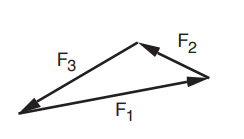
\includegraphics[width = 0.3\textwidth]{images/force_polygon.png}
    \caption{Force polygon}
    \label{fig:force-polygon}
\end{figure}

\begin{example}
    The graphical approach for equilibrium is particularly strong because of the sine theorem. Consider the example of a weight that is supported by a string in the following manner.
    
    \begin{figure}[h]
    \centering
    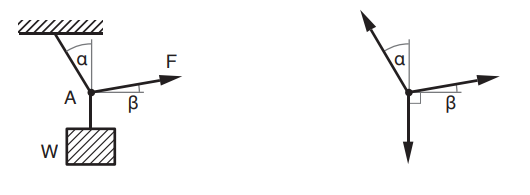
\includegraphics[width = 0.75\textwidth]{images/ex1.png}
    \caption{Three force equilibrium problem}
    \label{fig:ex-1}
    \end{figure}

    Because, of this, we can draw the following force polygon:

    \begin{figure}[h]
    \centering
    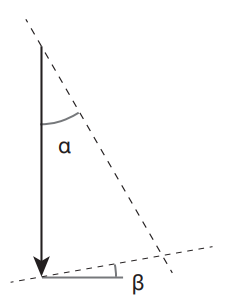
\includegraphics[width = 0.25\textwidth]{images/ex_2.png}
    \caption{Three force equilibrium problem - graphical solution}
    \label{fig:ex-2}
    \end{figure}

    The weight $\mathbf{W}$ acts vertically down, the tension $\mathbf{T}$ acts at an angle $\alpha$, and the force $\mathbf{F}$ acts at an angle $\frac{\pi}{2} - \beta$. By means of the sine theorem, we deduce that:

    \[ \frac{F}{\sin{\alpha}} = \frac{T}{\cos{\beta}} = \frac{W}{\cos{(\beta - \alpha)}} \]
\end{example}

Moreover, if a three-force member is in equilibrium and the forces are not parallel, they must be concurrent. Therefore, the lines of action of all three forces acting on such a member must intersect at a common point. Any single force is therefore the equilibrant of the other two forces. If there are more than three forces acting on a body, we can combine any two of them to further reduce the problem to only three forces.

\subsubsection{Distributed loads}

In reality, point forces cannot exist - as force is equal to pressure times area, a point force would require an infinite pressure (which does not make sense).

\begin{figure}[h]
    \centering
    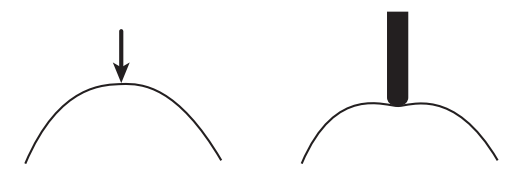
\includegraphics[width = 0.5\textwidth]{images/press.png}
    \caption{Point forces are in reality distributed}
    \label{fig:distributed_loads}
\end{figure}

All forces are therefore distributed over a finite area. When this area is relatively small, descriptions based on point forces can helpfully simplify the analysis without much loss of accuracy. However, some forces such as those applied to a body by fluids or gravitational attraction are distributed over a large enough area that we must account for their distribution in our analysis.

\subsubsection{Constant fluid pressure}

The pressure imposed on structures by stationary fluids is significant in applications such as pressure vessels or storage tanks.

\begin{theorem}[Pascal's law]
    The pressure $p$ at any given point in a stationary fluid is the same in all directions. Where the fluid meets a constraining surface, over any infinitesimal area, it imparts a force $\delta F = p \delta S$ normally to the surface.
\end{theorem}

Therefore, if our surface is a curve with unit normal vector $\mathbf{N}$, then:

\[ d\mathbf{F} = p (d\mathbf{S} \cdot \mathbf{N}) \mathbf{N} \]

However, if we have a curve, we need to perform a surface integration in order to obtain the total force acting upon it - this will be covered in the Structures course in part IB. We can, however, simplify our calculations by considering surfaces of unit width, and hence:

\[ \mathbf{F} = pL\mathbf{N} \]

\begin{example}
    For instance, let us consider the case of a curved surface in the shape of a semi-circle of unit width with a uniform pressure acting upon it. Then, for an infinitesimally small element of length:

    \[ dF = prd\theta \]

    And by means of integration:

    \[ F = \int_0^\pi prd\theta = \pi pr \]
\end{example}

\subsubsection{Hydrostatic loading}

Only in rare cases are structures loaded by a strictly uniform pressure - typically only in high pressure chambers. A more common form of pressure loading arises due to the weight of the fluid, which varies with depth and is known as hydrostatic pressure.

By means of equilibrium for a column of liquid, we can equate the Archimedic force with the force due to pressure:

\[ p(h)S = \rho Vg \]

This means that:

\[ p(h)S = \rho Sgh \iff p(h) = \rho gh \]

Now, consider the case where we have to replace a hydrostatic load from a height $h_1$ to a height $h_2$, with $h_1 < h_2$ with a point force. First, we can calculate the equivalent force. Suppose the area is of unit width. Then:

\[ F = \int_{h_1}^{h_2} \rho ghdh = \frac{1}{2}\rho g(h_2^2 - h_1^2) \]

And the equivalent point is calculated by taking moments about any of $h_1$ or $h_2$:

\[ Fh^* = \int_{h_1}^{h_2}\rho g h^2 dh \]

Implying that:

\[ h^* = \frac{\int_{h_1}^{h_2} \rho gh^2dh}{\int_{h_1}^{h_2} \rho g h dh} \]

\subsubsection{Gravity}

All structures are subject to forces due to gravity, whether through weights loading a structure or due to the self-weight of its components. These forces are always distributed, but to simplify analysis can often be treated as point forces at a particular location. We will not go into the same depth of analysis as in the Mechanics course. However, using the same result from it, we can see that:

\[ (x, y) = \left(\frac{\sum_i m_ix_i}{\sum_i m_i}, \frac{\sum_i m_iy_i}{\sum_i m_i}\right) \]

For a general lamina with uniform density and thickness, we know that $dm = \rho t dS$. The above equation can be thus restated as:

\[ (x, y) = \left(\frac{\int xdS}{\int dS}, \frac{\int ydS}{\int dS}\right) \]

Now, consider a general distributed force per length given by the function $f(x)$. We can then deduce, that in the most general case, the equivalent force is equal to:

\[ F = \int f(x)dx \]

And the equivalent point of application can be determine by taking moment:

\[ Fx^* = \int f(x)xdx \iff x^* = \frac{\int xf(x)dx}{\int f(x)dx} \]

\subsubsection{Contact forces}

Contact forces are reaction forces - knowing that two bodies are in contact tells us something about their displacement but gives us no information about the magnitude of the force between them. We can only find the contact force as the reaction to other applied forces, and the distribution and extent of these forces may vary over the history of loading as the contacting bodies interact.

In frictionless contact, a distributed force acts equally and oppositely on both bodies, similarly to the effect of static pressure on a body in previous subsections. Firctionless contact forces act normally to the contact interface, as shown below.

\begin{figure}[h]
    \centering
    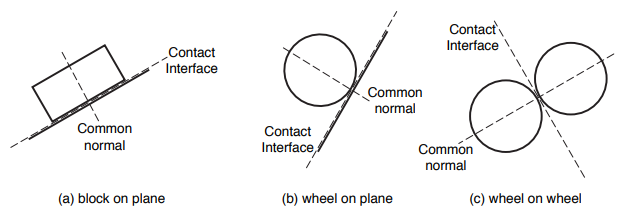
\includegraphics[width = 1\textwidth]{images/fcontact.png}
    \caption{The contact interface and common normal in frictionless contact}
    \label{fig:frictionless-contact}
\end{figure}

However, in reality we always have friction - this gives birth to a friction force $F = \mu N$ that acts normally to the common normal and that opposes movement. In structures, we will ditch the idea of friction being two forces, and instead we will introduce a reaction force $\mathbf{R}$ that represents the combined effects of the normal reaction and the friction force. Again, if there is no friction, we just have the common normal. If we have friction, the reaction starts to rotate by a certain angle. We distinguish between two cases:

\begin{enumerate}
    \item For static contact (no sliding), we must have that $F \leq \mu_sN$
    \item For dynamic contact (sliding between the bodies), we must have that $F = \mu_dN$
\end{enumerate}

Note that the static coefficient of friction is always higher than the dynamic coefficient of friction, i.e.:

\[ \mu_s > \mu_d \]

\begin{definition}[Angle of friction]
    The angle of friction is defined as:
    
    \[ \tan{\phi} = \frac{F}{N} \]
\end{definition}

Note that at any given point, it is true that the angle of friction is always less or equal to the static angle of friction, i.e.:

\[ \phi \leq \phi_s \]

There are different types of problems involving friction. If we have static contact, without impending motion, $F$ is not proportional to $N$, so $F$ must be found from consideration of equilibrium of the body only. However, it is true that $F < \mu_sN$ and $\phi < \phi_s$. If we have a static contact, on point of slipping problem, the angle of friction is equal to the angle of static friction, i.e. the friction force reaches is maximum value $F = \mu_sN$.

\subsubsection{Distributed friction}

\begin{example}[Sliding carpet]
    Find the force $T$ required to pull a carpet of length $L$ and weight $\omega$ per unit length at steady speed over a floor with coefficient of dynamic friction $\mu_d$.

    By considering equilibrium of a small section of carpet we deduce:

    \[ T(x) + dT = T(x) + \mu_dN \]
    \[ N = \omega dx \]

    Combining the two, we obtain:

    \[ dT = \mu_d \omega dx \iff T(x) = \mu_d \omega x + C\]

    We can determine the constant $C$ because we know that $T(0) = 0 \iff C = 0$. Hence:

    \[ T(x) = \mu_d \omega x \iff T = \mu_d \omega L \]
\end{example}

\begin{example}[Flexible belt on a pulley]
    A flexible belt is passed over a pulley as shown in the figure below. If the coefficient of static friction between the belt and the pulley is $\mu$, and $T_2 > T_1$, find the maximum ratio of $\frac{T_2}{T_1}$ before sliding occurs.

    \begin{figure}[h]
        \centering
        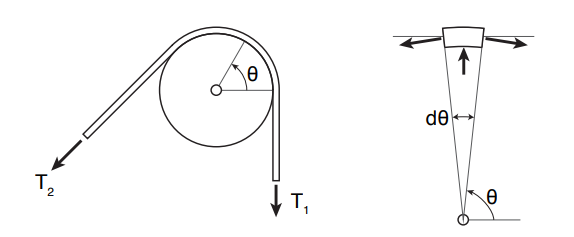
\includegraphics[width = 0.75\textwidth]{images/pulley.png}
        \caption{Belt passed over a pulley}
        \label{fig:pulley}
    \end{figure}

    By means of vertical equilibrium, we determine that:

    \[ R = 2T\sin{\frac{d\theta}{2}} + dT\sin{\frac{d\theta}{2}} \]

    Neglecting the terms with two differentials, and using the fact that $\sin{x} \to x$, as $x \to 0$, we deduce that:

    \[ R = Td\theta \]

    Horizontal equilibrium gives us:

    \[ dT = \mu R \]

    By combining both relationships:

    \[ dT = \mu T d\theta \iff \frac{1}{T} dT = \mu d\theta \]

    Denoting $\psi$ as the angle the belt moves over the pulley:

    \[ \int_{T_1}^{T_2} \frac{1}{T}dT = \int_0^\psi \mu d\theta \]

    Conversely:

    \[ \ln{\frac{T_2}{T_1}} = \mu\psi \]

    By exponentiating the result above, we deduce that:

    \[ \frac{T_2}{T_1} = e^{\mu\psi} \]

    This is a well known result, typically stated as:

    \[ \frac{T_{\text{big}}}{T_{\text{small}}} = e^{\mu\psi} \]
\end{example}

\subsubsection{Pin-joints}

Pin-joints are often used to connect structures to foundations. If the pin is frictionless, then the joint cannot apply a moment to the structures, which can be an advantage for structures such as trusses. A pin-joint applies a reaction force to the structure. As a result, like the contact forces of the previous section, it is only possible to find the magnitude and direction of the reaction at the pin-joint by solving the conditions of equilibrium in response to a set of applied loads. However, in contract with contact forces, the reaction force at a pin-joint can act in any direction.

\begin{figure}[h]
    \centering
    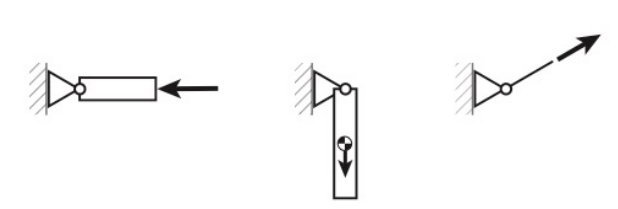
\includegraphics[width = 0.75\textwidth]{images/pinjoint.png}
    \caption{Pin-joint able to apply a reaction force in any given direction}
    \label{fig:enter-label}
\end{figure}

In analysing problems with pin-joints, it is assumed that they are frictionless and apply a point force to the structure. For pin joints, they restrict two degrees of freedom (they have both a vertical and a horizontal reaction).

\subsubsection{Roller supports}

A general three-dimensional body has six degrees-of-freedom: it would require six scalar
parameters to describe its motion, three linear translations and three rotations. The two-dimensional bodies considered in this course have three degrees-of-freedom. They can translate
horizontally or vertically (or in any other two non-parallel directions) and they can rotate.
Therefore, in order to ensure that a two-dimensional body, or structure, remains stationary it must
have three independent constraints.

However, were the beam supported by two pin-joints, as illustrated before, it would be over-constrained. The two pin-joints provide four constraints but the body has only three degrees of
freedom. As a result, it is not possible to find the reaction forces at the supports just be analysis of
equilibrium. To find all four reactions, we would need to know about the stiffness of the beam
and the supports, to find out how they interact. This is possible, but apart from complicating the
analysis, over-constraining a structure may have other unintended consequences. For example, if
a steel railway bridge is over-constrained, then thermal expansion or contraction of the bridge in
summer and winter would create additional and unwanted loading. 

For many structures, it is therefore important not to provide too many restraints. Therefore, if one
end of a beam is supported on a pin-joint, the other must have a different form of support. A
common solution is shown below a pin-joint is mounted on frictionless rollers. This
provides a vertical restraint on displacement but does not inhibit horizontal movement. Exactly
as with frictionless contact in the previous session, this form of support leads to a reaction force
in the direction of the common normal (i.e. perpendicular to the motion of the rollers). It is now
possible to solve the equilibrium of the beam just as we previously did it.

\begin{figure}[h]
    \centering
    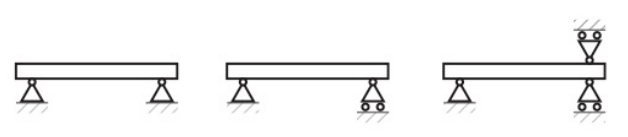
\includegraphics[width = 0.75\textwidth]{images/roller.png}
    \caption{\centering A beam on pin-joint supports: (a) over-constrained (b) with one pin-joint on rollers (c) with a double sided pin-joint on rollers}
    \label{fig:enter-label}
\end{figure}

\subsubsection{Built-in/"encastré" supports}

A roller-support constrains one degree of freedom of the displacement of a structure, while a pin-joint or simple support constrains two. The third important form of support therefore is one that
constraints all three degrees of freedom: linear displacement in either direction and rotation. This
is achieved by “building-in” the structure to the ground or some other reference at an “encastré”
(literally “en-cased”) support as illustrated below. This support – found in cantilevered
structures such as balconies or loading cranes that project out of the side of buildings, or in the
foundations of many concrete buildings – constraints all three degrees of freedom of a two-dimensional structure, so fully enforces equilibrium. The reaction forces provided by an encastré
support include two components of a force and a moment in reaction to the constraint on rotation.

\begin{figure}[h]
    \centering
    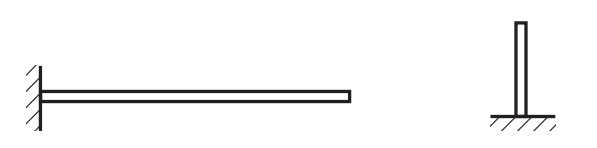
\includegraphics[width = 0.5\textwidth]{images/encastre.png}
    \caption{(a) horizontal and (b) vertical encastré supports}
    \label{fig:enter-label}
\end{figure}

\newpage

\subsection{Internal forces}

We will now focus our attention towards exploring how external forces are carried by structures.

\subsubsection{Pin-jointed trusses}

\begin{definition}[Pin-jointed truss]
    A framework of members joined at their ends is called a truss. A pin-jointed truss is a truss made up of struts that are joined at their ends by pin-joints.
\end{definition}

In this course we shall only consider a particular type of trusses, where all of the members lie in one plane - such frameworks are called two-dimensional/plane trusses.

\begin{figure}[h]
    \centering
    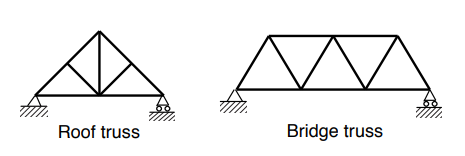
\includegraphics[width = 0.75\textwidth]{images/trusses.png}
    \caption{Example plane trusses}
    \label{fig:enter-label}
\end{figure}

We will make a few more assumptions before proceeding to analyzing trusses:

\begin{enumerate}
    \item We shall consider one type of connection only - the idealized frictionless pin, thus leading to pin-jointed plane trusses
    \item We will consider pin-jointed trusses subject to point loads applied at the joints only
    \item We assume straight, slender members
\end{enumerate}

Moreover, because the member is straight, if it were cut anywhere along its length, the internal force must equal the applied external force and is aligned along the members - exactly as if it were a string under tension. Thus, each members is in a state of pure tension or pure compression, i.e. it is an axial force member.

\subsubsection{Statically determinate frames}

In introducing the design of supports in a previous section of this course, we noted that structures should never be under- or over-constrained. For the two-dimensional structures we are considering in this course, they require three independent external restraints in order to remain fixed (the restraints must prevent rotation and translation in two directions). A similar issue arises with the design of the internal components of the structure: if they are under-connected, the structure will be a mechanism and may collapse without the application of any load; if they are over-connected, this may be a sign of inefficiency, but the analysis of the structure will be more difficult, as it is now statically indeterminate.

\begin{proposition}[Euler's conditions for structures]
    Let us consider a structure where $D$ is the number of dimensions, $j$ is the number of joints, $b$ is the number of bars, and $r$ is the number of restraints imposed upon the structure. Therefore:

    \begin{enumerate}
        \item If $Dj > b + r$, then the structure is a mechanism
        \item If $Dj = b + r$, then the structure is statically determinate
        \item If $Dj < b + r$, then the structure is statically indeterminate
    \end{enumerate}
\end{proposition}

However, this formula may fail in certain cases, such as the one below.

\begin{figure}[h]
    \centering
    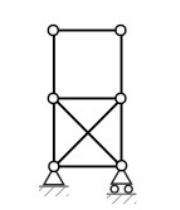
\includegraphics[width = 0.25\textwidth]{images/indet.png}
    \caption{Fail point of Euler's conditions}
    \label{fig:enter-label}
\end{figure}

The structure above is made of a mechanism and a statically indeterminate truss. Remember that for the formula to work, we need to only have our truss made out of triangles that do not overlap.

\subsubsection{Method of joints}

The method joints requires that we create a free-body diagram for each pin-joint of the truss. It provides a systematic way of calculating all the bar forces in a structure, purely by considering equiilibrium conditions at each point.

\begin{example}[Example usage of the method of joints]
    Consider the truss shown below. 

    \begin{figure}[h]
    \centering
    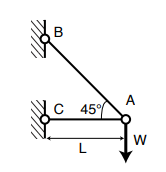
\includegraphics[width = 0.25\textwidth]{images/truss1.png}
    \caption{Method of joints example}
    \label{fig:enter-label}
    \end{figure}

    We begin by assuming all members are in tension, with the convention that tension is positive and compression is negative. By vertical equilibrium at $A$:

    \[ T_{\text{AB}}\frac{\sqrt{2}}{2} = W \iff T_{\text{AB}} = W\sqrt{2}\]

    Horizontal equilibrium gives:

    \[ W + T_{\text{AC}} = 0 \iff T_{\text{AC}} = -W \]

    Therefore, $AC$ is a compression member, while $AB$ is a tension member.
\end{example}

The method of joints is the better alternative when we need to find the forces in all members of a truss. However, there is another method if we need to find the tension in only a few members.

\subsubsection{Method of sections}

If we need to know the force in only one or two members of a truss, and the members are far from the supports, the method of joints involves a lot of work. In such cases, the method of sections can save a lot of effort.

In order to find the axial force in one specific bar only, we need to:

\begin{enumerate}
    \item Consider a continuous cut through the truss - it is useful to make the cut so that we only reveal a maximum of three members
    \item Consider the part of the truss that has less forces (external) acting upon it
    \item Reveal the forces and take moments such that two of the forces cancel
\end{enumerate}

\begin{example}
    Consider the plane pin-jointed truss below. Find the axial forces in bars $DF$ and $EG$.

    \begin{figure}[h]
    \centering
    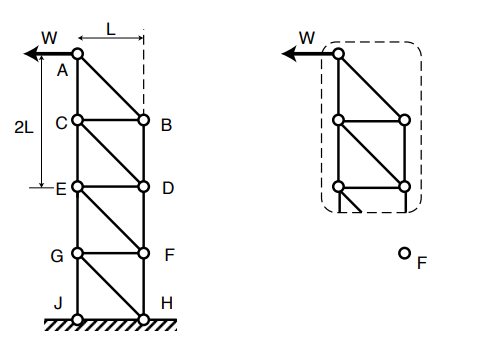
\includegraphics{images/truss3.png}
    \caption{Method of sections for a plane truss}
    \label{fig:enter-label}
    \end{figure}

    Consider the cut above. To find the reaction through $EG$, take moments about $F$ after revealing the three forces in the members:

    \[ T_{\text{EG}}L + 3WL = 0 \iff T_{\text{EG}} = -3W \]

    Now, to find the tension in the member $DF$, take moments about $E$:

    \[ T_{\text{DF}}L = 2WL \iff T_{\text{DF}} = 2W \]
\end{example}

Furthermore, there are three main simplifications we can use when analyzing pin-jointed trusses. Let us consider the figure below.

\begin{figure}[h]
    \centering
    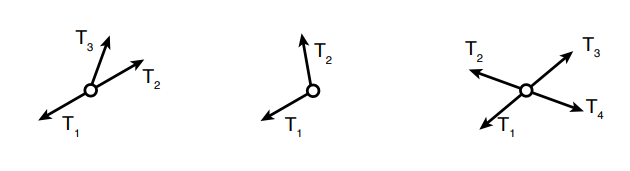
\includegraphics{images/truss4.png}
    \caption{Special cases}
    \label{fig:enter-label}
\end{figure}

For the first pin, $T_3 = 0$ and $T_1 = T_2$. For the second joint, because there is no external force applied, $T_1 = T_2 = 0$. For the last pin-joint, $T_1 = T_3$ and $T_2 = T_4$.

In general, when computing forces in all members of a truss, we first begin by calculating the external reactions, and then proceeding either by the method of sections or the method of joints. Consider the truss structure below.

\begin{example}
    Compute the force in the member $DE$ due to a vertical load $W$ at $E$.

    \begin{figure}[h]
    \centering
    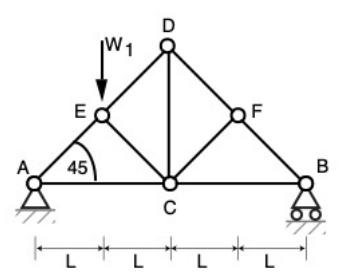
\includegraphics[width = 0.4\textwidth]{images/truss5.png}
    \caption{Truss with a single vertical load}
    \label{fig:enter-label}
    \end{figure}

    Since $A$ is pin-jointed, there will be two reaction forces $V_A$ and $H_A$. $B$ is a roller support, so we only have a vertical reaction $V_B$. By horizontal equilibrium, $H_A = 0$. Taking moments about $A$:

    \[ WL = 4V_BL \iff V_B = \frac{W}{4} \]
 
    By means of vertical equilibrium, the reaction at $A$ is given by:

    \[ V_A = W - \frac{W}{4} = \frac{3W}{4} \]

    Consider a cut going through $DE$, $EC$ and $AC$ and take the left side of the truss. Take moments about $C$:

    \[ T_{\text{DE}} L\sqrt{2} + 2V_BL = 0 \iff T_{\text{DE}} = -W\frac{\sqrt{2}}{4} = -\frac{W}{2\sqrt{2}} \]
\end{example}

\subsubsection{Superposition}

Consider a plane truss to which we apply a sequence of loads $W_1, W_2, \dots, W_n$. Let us consider that there exists constant $\lambda_k$ so that upon imposing the load $W_k$, the axial force in a chosen member is given by $\lambda_kW_k$. Therefore, the force $T$ due to applying all loads at once is given by:

\[ T = \sum_{k = 1}^n \lambda_kW_k \]

Hence, plane trusses form a linear system. Furthermore, the conditions upon the behavior of a truss is linear are:

\begin{enumerate}
    \item The material of the truss remains in the linear elastic range
    \item The geometry changes, i.e. the distortion of the structure caused by the loads is small - hence, the equilibrium equations written in the undeformed configuration are also valid after the structure has deformed
\end{enumerate}

Note that these conditions are inherently true for most structures made out of metal.

\subsubsection{Symmetry}

Many structures are symmetric - both for aesthetic reasons and to simplify their production. Symmetry always leads to a reduction in the effort of analyzing a structure, and therefore should be always exploited.

A common example of symmetry for trusses is when they are symmetric about a vertical centre-line, and are said to have "mirror symmetry". If a truss has symmetry about a line, and the loads are symmetric about the same line, then it follows that the bar tensions (and support reactions) must also be symmetric about that line.

\begin{figure}[h]
    \centering
    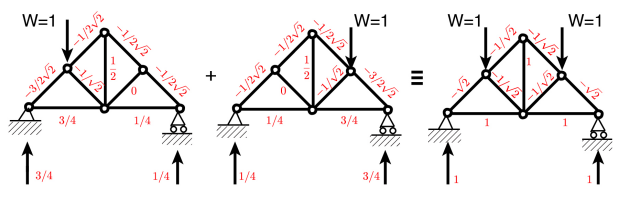
\includegraphics{images/symmetry.png}
    \caption{Symmetric loading on a truss leads to symmetric internal forces}
    \label{fig:enter-label}
\end{figure}

Furthermore, for a symmetric structure it is always possible, and sometimes even convenient, to represent any set of applied loads by superposing a symmetryc and an anti-symmetric set of loads, as shown below:

\begin{figure}[h]
    \centering
    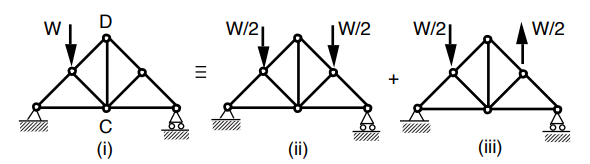
\includegraphics{images/symmetry2.png}
    \caption{Symmetric/anti-symmetric load combination}
    \label{fig:enter-label}
\end{figure}

\subsubsection{Shear forces and bending moments}

The previous sections explored how external forces acting on a pin-jointed planar truss can be translated into internal forces. The assumption of frictionless pin-joints and the use of only straight members and nodal loading ensured that all the members of the truss were axially loaded, so the internal forces must be tension or compression aligned with the member. The figure below shows that if any of these requirements is not met, then when a free-body diagram is created for a section of the member, it cannot be held in equilibrium by a single axial force.

\begin{figure}[h]
    \centering
    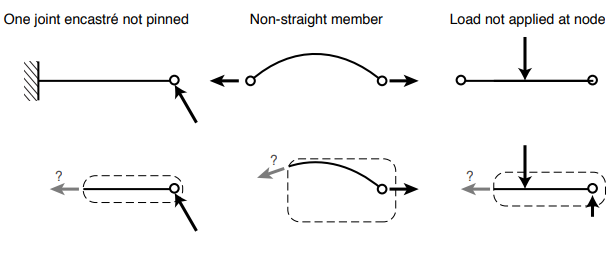
\includegraphics{images/shear1.png}
    \caption{Three variants of axial members which cannot maintain equilibrium}
    \label{fig:enter-label}
\end{figure}

\begin{definition}[Shear force and bending moment]
    It is then clear that equilibrium can only be maintained if at the point where the member was cut by the method of sections, a force perpendicular to the axial force and a moment are applied. These, respectively, are known as the shear force and the bending moment.
\end{definition}

\subsubsection{Arches}

Arches occur widely in structural engineering - the structural benefit of arches is that their shape can be chosen so that the internal forces in the arch are mainly in compression. This is important for stone masonry - the joints between stone blocks are typically strong in compression, but weak in tension. It can also be useful in metal structures, where reduced bending moments allow the use of lighter members.

\begin{example}
    Consider the following triangular arch, that supports a weight $W$ and that is comprised of two rigid bars, each of length $2L$, inclined at $30^\circ$ to the horizontal, pinned together at $B$ and to vertical walls at $A$ and $C$ as shown below.

    \begin{figure}[h]
        \centering
        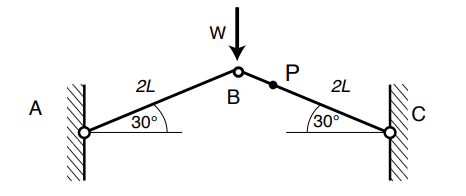
\includegraphics{images/arch.png}
        \caption{Triangular arch example}
        \label{fig:enter-label}
    \end{figure}

    Taking moments about $A$ and by then applying vertical equilibrium, we obtain that $V_A = V_C = \frac{W}{2}$. By taking a cut about the segment $AB$ at $B$ and taking moments about $B$, we can obtain that:

    \[ 2LV_A\frac{\sqrt{3}}{2} = H_AL \iff H_A = V_A\sqrt{3} = \frac{W\sqrt{3}}{2} \]
\end{example}

Note that arches rely upon their supports, called abutments, to resist lateral movement. If abutment movement is significant, the arch may deform or even collapse.

\subsubsection{Segmented arches}

Segmented arches are those made of blocks, such as stone arches in bridges and churches. Generally, they cannot carry tensile loads at joints, and three assumptions are typically made in order to analyze them:

\begin{enumerate}
    \item The blocks are infinitely strong (no compression failure)
    \item The block interfaces are unable to carry bending moments (no tensile capacity)
    \item Block interfaces have infinite friction (there is no lateral sliding along the interfaces)
\end{enumerate}

In the simplest terms, we can deduce if a segmented arch is stable if we can draw reaction lines from the abutments to the point load, such that the lines of action of the two reactions remain within the structure.

\begin{figure}[h]
    \centering
    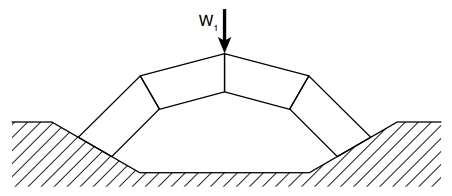
\includegraphics[width = 0.4\textwidth]{images/segarch1.png}
    \caption{Segmented arch under two different loads (1)}
    \label{fig:enter-label}
\end{figure}

\begin{figure}[h]
    \centering
    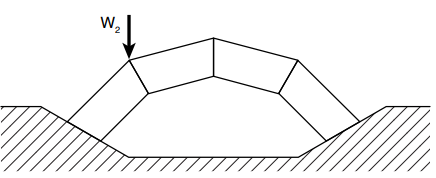
\includegraphics[width = 0.4\textwidth]{images/segarch2.png}
    \caption{Segmented arch under two different loads (2)}
    \label{fig:enter-label}
\end{figure}

In the above two figures, we have the same arch subjected to two different loads. In the first case, the arch is stable - we can easily draw abutment reactions such that they intersect at $W_1$. However, for the load $W_2$, the structure would collapse, because there is no way for us to draw a reaction from the right side of the arch that intersects with $W_2$, unless it goes outside the structure.

\subsubsection{Continuous arches}

Continuous (thin) arches use bending moment capacity to resist alternate loading conditions, instead of geometric thickness. These arches are always described by an equation of the type $y = y(x)$ that gives us the height of the arch at a horizontal distance $x$ away from the centre $O$.

\begin{example}
    The arch bridge illustrated below carries a uniform load $\omega$ per unit horizontal length and has parabolic shape $y = d\frac{x^2}{L^2}$. Find the abutment reactions, and the bending moment at a distance $x$ from the origin.

    \begin{figure}[h]
    \centering
    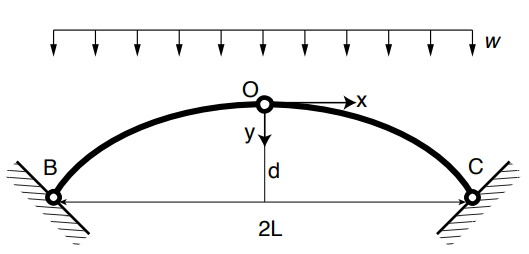
\includegraphics{images/contarch1.png}
    \caption{Pin-jointed parabolic continuous arch with uniformly distributed loading}
    \label{fig:enter-label}
    \end{figure}

    First, we need to find the abutment reactions. Let use replace the distributed load by a point load $W = 2\omega L$ at the origin. Taking moments about $B$:

    \[ 2\omega L^2 = 2V_CL \iff V_C = \omega L \]

    By vertical equilibrium, the vertical reaction at abutment $B$ is $V_B = \omega L$. Now, consider a cut at $O$ and take moments about $O$. Keep in mind that we now have a distributed load $\omega L$ acting at $\frac{L}{2}$ from the origin.

    \[ \omega \frac{L^2}{2} + Hd - \omega L^2 = 0 \iff Hd = \frac{\omega L^2}{2} \]

    Therefore, the horizontal reactions are given by:

    \[ H = \frac{\omega L^2}{2d} \]

    Now, we can consider a cut at a distance $x$ away from the origin. We can now calculate the bending moment:

    \[ M(x) + Hd\frac{x^2}{L^2} - \frac{\omega x^2}{2} = 0 \iff M(x) = \frac{\omega x^2}{2} - \frac{\omega x^2}{2} \iff M(x) = 0 \]
\end{example}

This is an interesting result - for a continuous arch with a uniformly distributed weight per horizontal length, there is no bending moment anywhere - the arch effectively behaves as if any point on it is a pin-joint. 

Furthermore, consider a continuous arch where on one side we have a force $W$, and the other side is unloaded, as in the figure below.

\begin{figure}[h]
    \centering
    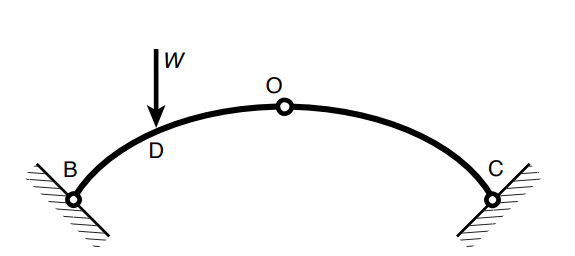
\includegraphics{images/contarch2.png}
    \caption{General three-pin parabolic arch with a single point load}
    \label{fig:enter-label}
\end{figure}

On the right side $OC$, we only have the reactions at $O$ and $C$ acting - so they must be colinear. Because of this, we know that the reaction at $O$ acts parallel to $OC$. Therefore, the reaction at $B$ acts through the point of intersection between the line of action of $W$ and the line $OC$. Therefore:

\begin{enumerate}
    \item The abutment reaction at $C$ is in the direction $OC$
    \item The maximum bending moment in $OC$ is where the tangent to the arch is parallel to $OC$
    \item The maximum bending moment in $OB$ is at point $D$
\end{enumerate}

\subsubsection{Stress}

When a component made of metal or other stiff material is loaded by external forces, the component acts as a spring, changing shape under the loads. For relatively small changes from their equilibrium separation, the force between two atoms changes nearly linearly, and this is the basis of Hooke's law.

In two-dimensional problems, the state of stress has the three components illustrated in the figure below. The two direct stresses $\sigma_x$, $\sigma_y$ tend to stretch or compress the material along an axis. The shear stress $\tau_{xy}$ tends to shear the material from a small square to a rhomboid shape.

\begin{figure}[h]
    \centering
    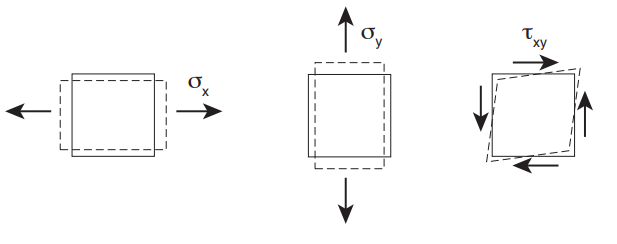
\includegraphics{images/stress1.png}
    \caption{The three components of stress in two-dimensions}
    \label{fig:enter-label}
\end{figure}

The stresses have units of force per area, so the internal forces (stress) can be related to external loads by integrating them with respect to area, over the boundary influenced by the load. This is illustrated below for a small rectangular lamina in a state of uniform stress.

\begin{figure}[h]
    \centering
    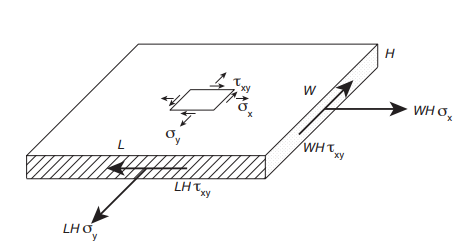
\includegraphics{images/stress2.png}
    \caption{The relationship between external forces and the internal state of stress}
    \label{fig:enter-label}
\end{figure}

The units of stress are the same as those of pressure. However, pressure has no direction: at any point in a fluid, it acts identically in all directions. In contrast, the components of the state of stress have specific directions (as indicated by the subscripts). The state of stress must therefore always be stated with respect to a set of axes. For a given components under constant external loads, the state of stress varies as the axes rotate. 

General stress analysis is largely left to Part II courses, but the concept is central to all of structural analysis, because the state of stress is the most general description of the internal loads within a body. In this section, we will consider only conditions which lead to a uniform state of stress, as well as conditions that allows us to describe the internal state of a beam bent under the action of external loads.

\subsubsection{Thin walled shells with uniform stress}

Pressure vessels, such as balloons, pipelines, etc. are designed to carry internal or external pressure. Furthermore, we will only consider thin-walled pressure vessels, where it can be assumed that the stress distribution is uniform throughout the thickness. Also, we will consider vessels with axi-symmetric shape, such as spheres or cylinders, for which the stress distribution is uniform along any circumferential or longitudinal section.

\begin{figure}[h]
    \centering
    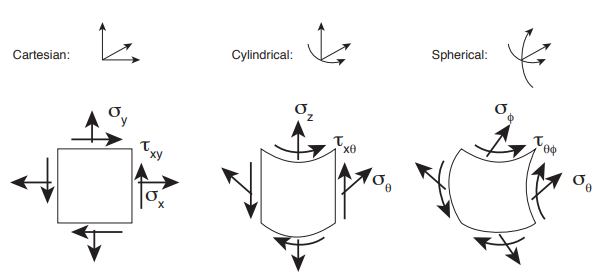
\includegraphics{images/stress3.png}
    \caption{Components of the state of stress for thin-walled vessels}
    \label{fig:enter-label}
\end{figure}

In the above figure, along the length (height) of the cylinder, $\sigma_z$ is the longitudinal stress, and $\sigma_\theta$ is the circumferential stress. Furthermore, $\sigma_\theta$ is the hoop stress for a spherical object.

The stress in such a pressure vessel is found using the method of sections. As with the analysis of trusses and beams, a cut is made around one section of the loaded pressure vessel, typically a plane-cut through the vessel in some direction. Asserting equilibrium across this plane, the external force must equal the internal force found as the stress in the wall of the pressure vessel acting normal to the plane multiplied by the area of the cut surface of the vessel, i.e.:

\[ pS_{\text{projected}} = \sigma_{\text{normal}}S_{\text{cut}} \]

Using the convention that tensile stress is positive.

\begin{example}[Hoop stress in a sphere]
    Consider a sphere with radius $R$ and thickness $t$.

    \begin{figure}[h]
        \centering
        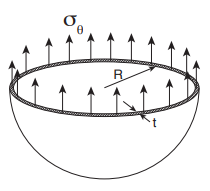
\includegraphics[width = 0.15\textwidth]{images/stress4.png}
        \caption{A free-body diagram for half a pressured spherical balloon}
        \label{fig:enter-label}
    \end{figure}

    Therefore:

    \[ \pi pR^2 = \sigma_\theta 2\pi Rt \iff \sigma_\theta = \frac{pR}{2t} \]

    This is the hoop stress in a sphere pressure vessel.
\end{example}

\begin{example}[Circumferential stress in a cylinder vessel]
    Consider a cylinder of radius $R$ and thickness $t$, as shown below.

    \begin{figure}[h]
        \centering
        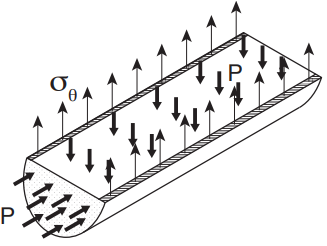
\includegraphics[width = 0.45\textwidth]{images/stress5.png}
        \caption{A long cylinder subject to internal pressure}
        \label{fig:enter-label}
    \end{figure}

    We can apply the identity above again:

    \[ 2pRL = 2\sigma_\theta Lt \iff \sigma_\theta = \frac{pR}{t}  \]
\end{example}

\begin{proposition}[Two-dimensional stress equations]
    For a two-dimensional object, we can deduce that the state of stress obeys the following relationships:

    \[ \frac{\partial \sigma_x}{\partial x} + \frac{\partial \tau_{xy}}{\partial y} + b_x = 0 \]
    \[ \frac{\partial \sigma_y}{\partial y} + \frac{\partial \tau_{xy}}{\partial x} + b_y = 0 \]
\end{proposition}

\newpage

\subsection{Deflection}

Having now explored the equilibrium of external forces and their translation into internal forces within a structure, we can now begin to consider how the structure deforms. Although structures may fail due to limits to their strength, many designs are limited more by deflection. 

\subsubsection{Cables and bar extensions}

Cables, strings, ropes and chains are able to carry uniaxial tension, but they are unable to carry compression or bending, as they have negligible bending stiffness. As a result, it is a good assumption that the tension at any point acts in the direction of the tangent to the cable at that point.

\begin{example}
    Consider the following structure below. Our goal is to find a relationship between $W_1$, $W_2$ and $\alpha$.

    \begin{figure}[h]
        \centering
        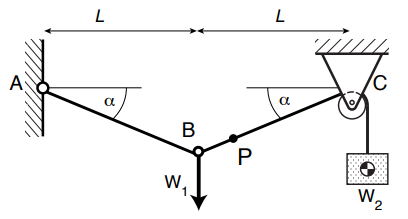
\includegraphics{images/cable1.png}
        \caption{Rope bridge supported by pulley and weight}
        \label{fig:enter-label}
    \end{figure}

    For the right side of the structure, $T_{\text{BC}} = W_2$. Now, by means of a force polygon, since $T_{\text{AB}} = T_{\text{BC}}$, we deduce that:

    \[ \sin{\alpha} = \frac{W_1}{2W_2} \]
\end{example}

\subsubsection{Shape of a cable subject to distributed loads}

Consider a shallow cable with mid-point displacement $d << L$. We will now derive the shape of the cable by making use of two methods. Let us suppose that the load has a weight distribution of $\omega$ N/m.

\begin{figure}[h]
    \centering
    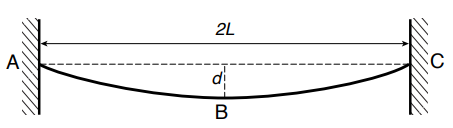
\includegraphics[width = 0.5\textwidth]{images/cable2.png}
    \caption{Cable subject to uniformly distributed load}
    \label{fig:enter-label}
\end{figure}

By taking moments about $A$ and then by means of a vertical equilibrium arguments, we deduce that $V_A = V_C = \omega L$.

Now, consider a cut through $B$ and take moments about point $B$:

\[ V_AL = Hd + \frac{\omega L^2}{2} \]

This is equivalent to:

\[ \omega L^2 = Hd + \frac{\omega L^2}{2} \iff Hd = \frac{\omega L^2}{2} \iff H = \frac{\omega L^2}{2d} \]

Now, consider a cut at a random distance $x$ from point $B$. By taking moments about $X$:

\[ \omega x \frac{x}{2}  = Hy \iff \frac{\omega x^2}{2} = \frac{\omega L^2}{2d}y \]

Therefore, we obtain that:

\[ y(x) = d\left(\frac{x}{L}\right)^2 \]

Note that we measure $y$ with respect to $B$. In general, we consider the origin as the point where the cable sags the most. We always have to consider the cut with respect to the origin.

Now, we can also consider the forces on a small elements of cable at a distance $x$ to the right and $y$ above the centre $B$. By horizontal equilibrium:

\[ H = H + \delta H \iff \delta H = 0 \]

By vertical equilibrium:

\[ V + \delta V = V + \omega \delta x \iff \delta V = \omega\delta x \iff \frac{\delta V}{\delta x} = \omega \]

Furthermore, $\frac{\delta y}{\delta x} = \frac{V}{H}$. By taking both of these into the limit, we deduce that $\frac{dV}{dx} = \omega$ and $\frac{dy}{dx} = \frac{V}{H} \iff V = H\frac{dy}{dx}$. By differentiating this:

\[ \frac{dV}{dx} = H\frac{d^2y}{dx^2} \iff \omega = H\frac{d^2y}{dx^2} \]

Therefore:

\[ \frac{d^2y}{dx^2} = \frac{\omega}{H} \]

By solving this differential equation, and setting the boundary conditions as $y(0) = 0$ and $\frac{dy}{dx} = 0$ at $x = 0$, we can deduce the same equation as before. 

\begin{proposition}[Length of a cable]
    Suppose we have a cable of shape $y = y(x)$ that spans over a horizontal length $L$. Then, the total length of the cable is given by:

    \[ l = \int_0^L \sqrt{1 + \left(\frac{dy}{dx}\right)^2}dx \]
\end{proposition}

Also note that the tension in the string at any given point is $T = \sqrt{T_x^2 + T_y^2}$.

\subsubsection{Strains, Hooke's law and bar extensions}

The Young's Modulus $(E)$ is a material property, and the relationship that governs the force and the extension is given by:

\[ F = \frac{ES_0}{L_0}\Delta L \]

\begin{definition}[Stress]
    We define the stress as $\sigma = \frac{F}{S}$. This is the same as previously defined in the section where we analyzed pressure vessels.
\end{definition}

\begin{definition}[Strain]
    The strain (in one dimension) is the relative elongation of the member, i.e.:

    \[ \epsilon = \frac{\Delta L}{L_0} \]
\end{definition}

Furthermore, Hooke's law  can be written as:

\[ \sigma = E\epsilon \]

Also, the extension of any member can be calculated as:

\[ e = \frac{FL_0}{ES_0} \]

Moreover, members can extend (and contract) due to temperature. Experiments have shown that the one-dimensional thermal strain $\epsilon_T$ in a long, straight, slender member due to a uniform temperature change $\Delta\theta$ can be predicted using the formula:

\[ \epsilon_T = \alpha\Delta\theta \]

Therefore, the total strain in a member is:

\[ \epsilon = \frac{F}{ES_0} + \alpha\Delta\theta \]

And lastly, we can deduce that the total extension experienced by the member is:

\[ e = \frac{FL_0}{ES_0} + \alpha\Delta\theta L_0 \]

\subsubsection{Displacement diagrams}

We will now analyze what happens when all members of a structure change length. However, we make two assumptions: the extensions are very small in comparison to the length of each member. Therefore, we assume that:

\begin{enumerate}
    \item All extensions are parallel to the original member
    \item All rotations are perpendicular to the original member
\end{enumerate}

Consider a general truss structure. The general procedure to draw a displacement diagram and deduce the extensions of each member is:

\begin{enumerate}
    \item Select the origin pole of the displacement diagram so that the displacement of all other points can be measured relative to $O$; note that the origin must be a point (or multiple points) that do not change position
    \item Draw extensions for members $P_iP_k$ and $P_jP_k$
    \item Draw the rotations for the above members
    \item Intersect them in order to deduce the position of point $P_k$
\end{enumerate}

In general, when given a truss structure, we must first calculate all the extensions my first computing the bar forces and then using Hooke's law. Afterwards, we can draw the displacement diagram. Consider the below truss structure, with the shown extensions.

\begin{figure}[h]
    \centering
    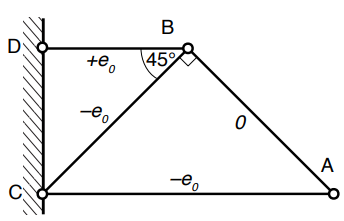
\includegraphics[width = 0.5\textwidth]{images/displacement1.png}
    \caption{Truss structure with displacements}
    \label{fig:enter-label}
\end{figure}

It is obvious that in this case points $D$ and $C$ do not move. Therefore, we choose them as the origin. Now, we can draw the following displacement diagram:

\begin{figure}[h]
    \centering
    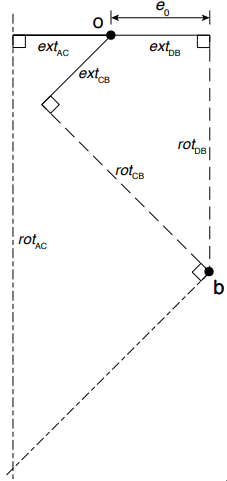
\includegraphics[width = 0.25\textwidth]{images/displacement2.png}
    \caption{Displacement diagram}
    \label{fig:enter-label}
\end{figure}

\subsubsection{Displacement for symmetric structures}

Consider the following structure:

\begin{figure}[h]
    \centering
    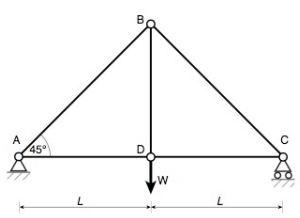
\includegraphics{images/displacement3.png}
    \caption{Symmetric structure}
    \label{fig:enter-label}
\end{figure}

As we can observe, the above structure is symmetric about the $DB$ vertical member. For this reason, $DB$ needs to remain vertical - it cannot rotate. For this reason, we can choose $D$ as the origin of our displacement diagram, and immediately draw the extension of member $DB$ to find $B$ vertically above $D$.

\subsubsection{Real work}

The principle of conservation of energy states that in a closed system, the total energy is conserved over time. The experiment of a mass hung on a wire is now repeated. Considering this as a closed system, when the weight is applied to the wire, the potential energy lost by the weight is taken up as energy stored in the wire due to its stretching, and any kinetic energy due to the weight moving.

\begin{proposition}[Real work for plane trusses]
    Consider a truss structure with forces $\mathbf{F}_i$, $1 \leq i \leq n$ applied to it, leading to displacements $\mathbf{d}_i$, tensions $\mathbf{T}_j$ and extensions $\mathbf{e}_j$. Hence:

    \[ \sum_i \mathbf{F}_i \cdot \mathbf{d}_i = \sum_j \mathbf{T}_j \cdot \mathbf{e}_j \]

    And because the extensions in the bars are parallel to each member (and thus parallel to each tension):

    \[ \sum_i \mathbf{F}_i \cdot \mathbf{d}_i = \sum_j T_je_j \]
\end{proposition}

For instance, if we would apply a unit load of size $1$ (this is just to simplify our calculations, as a load of size $1$ actually means $W$) at point $D$ in the truss above, we can deduce that:

\[ \delta_{D}^V = 2.9 \frac{WL}{AE} \]

Note that real work is applied when we want to calculate the displacement of a point in the direction of the force applied to it. If there is no force applied to it, however, we must use virtual work.

\subsubsection{Virtual work}

\begin{proposition}[Virtual work]
    Suppose we wish to find the displacement of a joint $P_i$ due to a load applied at joint $P_j$. To do this, we will first compute all the real extensions imposed by the load at joints $P_j$. Afterwards, we impose a unit load in the direction (either horizontal or vertical) of the displacement, in order to find the virtual set of tensions $T^*_j$. Therefore:

    \[ \sum_i \mathbf{F}_i^* \cdot \mathbf{d}_i = \sum_j T_j^* e_j \]

    The stars indicate that we have a set of virtual forces and tensions, and a set of real extensions and displacements. We may also utilize a real set of forces and impose a solid body rotation of an angle $\psi$ in order to deduce the force in certain members. However, this is not the most effective way to calculate forces, as all it does is that it just mimics moments with an extra headache added. We therefore use virtual work to determine the extensions of certain joints, and the method of sections/method of joints if we wish to determine the forces in certain members.
\end{proposition}

\subsubsection{Structural optimisation}

Suppose we have a plane structure and a pin-joint $P_k$ - we want to reduce the deflection (horizontal or vertical) under this loading by adding some mass (i.e., volume) to one of the bars - which one do we choose? By means of virtual work, we know that:

\[ \delta_{P_k} = \sum_j T_j^* \frac{T_jL_j}{A_jE} \]

However, we note that $V_j = A_jL_j \iff \delta_{P_k} = \sum_j T_j^* \frac{T_jL_j^2}{V_jE}$ is the displacement of point $P_k$ under this loading.

Let us fix a random member $j$ and take the partial derivative of the above expression with respect to the volume of the bar:

\[ \frac{\partial P_k}{\partial V_j} = -T_j^* \frac{T_jL_j^2}{V_j^2E} = -T_j^* \frac{T_j}{A_j^2E}  \]

Therefore, the bar for which the deflection would be minimized if we added mass to it is the bar for $j, 1 \leq j \leq n$ for which $\frac{\partial P_k}{\partial V_j}$ is minimized (or the most negative). Conversely, the bar for which the same partial derivative is maximized, the deflection is the biggest.

\newpage

\subsection{Equilibrium of beams}

So far, we have only analyzed truss structures, where each of the members carries only an axial load. However, there are many structures where assuming only axial loads will simply not work. One such example are beams.

\begin{definition}[Simply supported beam]
    We say that a beam is simply supported if it is long and slender, and the end supports:
    \begin{enumerate}
        \item Prevent any vertical movement
        \item Allow rotation
        \item Only one of the supports is able to prevent horizontal movement
    \end{enumerate}
\end{definition}

\begin{figure}[h]
    \centering
    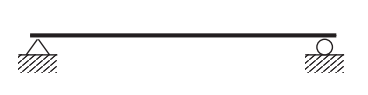
\includegraphics[width = 0.5\textwidth]{images/simply.png}
    \caption{Simply supported beam}
    \label{fig:enter-label}
\end{figure}

\begin{definition}[Cantilever beam]
    We say that a beam is cantilevered is the end support:
    \begin{enumerate}
        \item Prevents vertical movement
        \item Prevents horizontal movement
        \item Prevents rotation
    \end{enumerate}
\end{definition}

\begin{figure}[h]
    \centering
    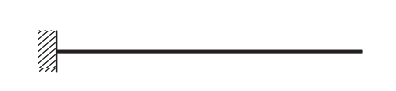
\includegraphics[width = 0.5\textwidth]{images/cantilever.png}
    \caption{Cantilever beam}
    \label{fig:enter-label}
\end{figure}

In order to analyze such structures, we proceed as we did before, making cuts at various distances and analyzing the forces/moments to the left/right of the cut.

\begin{proposition}[Hypotheses]
    For our theory to be accurate, we must make a few assumptions regarding the beams/structures we are going to analyze:
    \begin{enumerate}
        \item All bending moments are too small to either break or permanently bend the beam
        \item We only consider two-dimensional situations, although all concepts can be generalized into three dimensions
        \item We assume that the structure does not deflect significantly under load, and we can consider equilibrium in the original configuration
    \end{enumerate}
\end{proposition}

Furthermore, our sign convention will be the same as previously:

\begin{figure}[h]
    \centering
    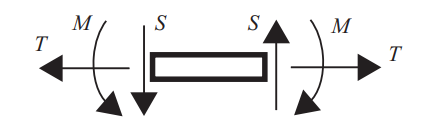
\includegraphics[width = 0.5\textwidth]{images/signconvention.png}
    \caption{Sign convention}
    \label{fig:enter-label}
\end{figure}

\begin{example}
    Find the shear force and bending moment in the following cantilevered beam.

    \begin{figure}[h]
        \centering
        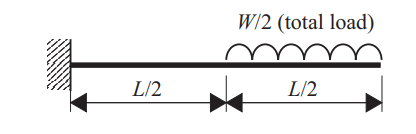
\includegraphics[width = 0.5\textwidth]{images/examplebeam.png}
        \caption{Partially loaded beam}
        \label{fig:enter-label}
    \end{figure}

    Consider a cut a distance $x$ away from the support end, firstly on $x \geq \frac{L}{2}$. Therefore, the bending moment is:

    \[ M(x) = \frac{W(L-x)^2}{2L} \]

    For $x \leq \frac{L}{2}$, the bending moment is equal to:

    \[ M(x) = \frac{W}{2}\left(\frac{L}{2} - x + \frac{L}{4}\right) \]

    Hence, the bending moment distribution is:

    \[ M(x) = \begin{cases}
        \frac{W(L-x)^2}{2L}, x \geq \frac{L}{2} \\
        \frac{W}{2}\left(\frac{3L}{4} - x\right), x \leq \frac{L}{2}
    \end{cases} \]

    The shear force will be negative due to our convention, equal to:

    \[ S(x) = \begin{cases}
        -\frac{W}{2}, x \leq \frac{L}{2} \\
        -\frac{W(L - x)}{L}, \frac{L}{2} < x \leq L
    \end{cases} \]
\end{example}

These can then be plotted on shear force and bending moment diagrams respectively to show the loading parameters of the said structure.

\newpage

\subsubsection{Differential equilibrium}

Let us consider an infinitesimally small piece of a beam in equilibrium.

\begin{figure}[h]
    \centering
    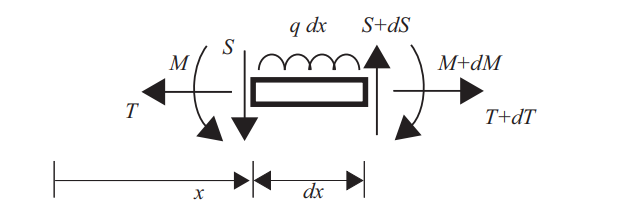
\includegraphics[width = 0.75\textwidth]{images/diffeq.png}
    \caption{Differential equilibrium}
    \label{fig:enter-label}
\end{figure}

Horizontally, we deduce that:

\[ dT = 0 \]

Therefore, $T$ is a constant; this is valid as long as there is no axial loading. Vertically:

\[ dS = qdx \iff q = \frac{dS}{dx} \]

By taking moments:

\[ dM = Sdx + \frac{1}{2}dSdx \]

Neglecting $dSdx$ due to it being too small, we deduce that $dM = Sdx$, hence:

\[ S = \frac{dM}{dx} \]

\begin{theorem}[Differential equilibrium]
    For the standard sign convention we have considered so far, the differential equations of equilibrium are:

    \[ q = \frac{dS}{dx} \iff S = \frac{dM}{dx} \]
\end{theorem}

This relationship allows us to gain intuition into two different consequences:

\begin{enumerate}
    \item If the loading on a beam is purely done by point loads, then the shear force is constant between two consecutive point loads, while the bending moment varies linearly
    \item If the loading on a beam is purely done by distributed loads (linearly), then the shear force varies linearly between two consecutive loading conditions, while the bending moment varies quadratically
\end{enumerate}

\newpage

\subsection{Deflection of straight elastic beams}

\begin{definition}[Curvature]
    The curvature of a plane curve is best defined in the intrinsic coordinate system $(s, \psi)$, as shown beloww. The curvature at a point of the curve is given by:

    \[ \kappa = \frac{d\psi}{ds} \]
\end{definition}

\begin{figure}[h]
    \centering
    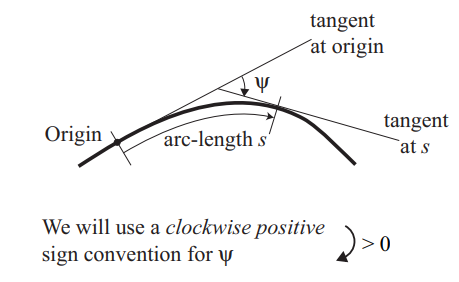
\includegraphics[width = 0.5\textwidth]{images/curvature.png}
    \caption{Curvature}
    \label{fig:enter-label}
\end{figure}

Furthermore, there exist a relationship, as described in Mechanics, between the curvature and the radius of curvature, i.e.:

\[ \rho = \frac{1}{\kappa} \] 

\begin{proposition}[Curvature equivalence]
    Due to our assumption that beams deflect by very small amounts, we can approximate that $ds \approx dx$, and hence:

    \[ \kappa = \frac{d\psi}{dx} \]
\end{proposition}

Now, consider the figure below, showing the full deflection-rotation of a beam.

\begin{figure}[h]
    \centering
    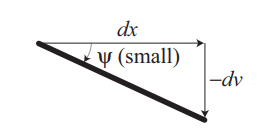
\includegraphics[width = 0.35\textwidth]{images/deflect.png}
    \caption{Deflection equivalence}
    \label{fig:enter-label}
\end{figure}

Above, we considered an infinitesimally small element of beam. We can observe, from the small angle approximation, that:

\[ \psi = -\frac{dv}{dx} \]

Therefore, we deduce the following:

\[ \kappa = \frac{d\psi}{dx} = \frac{d}{dx}\left(-\frac{dv}{dx}\right) = - \frac{d^2v}{dx^2}\]

\begin{theorem}[Moment-deflection equivalence]
    Let us consider a straight elastic beam with bending moment distribution $M = M(x)$. Therefore:

    \[ M = EI\Delta\kappa  \]

    In the case of no initial curvature on the beam, the relationship degenerates into:

    \[ M = EI\kappa \iff M = -EI\frac{d^2v}{dx^2} \]
\end{theorem}

The relationship above will be proved in a later section. The idea, however, is simple - in order for us to be able to find the deflection/deflected shape of a beam, we first must find the bending moment distribution, then deduce what $\frac{d^2v}{dx^2}$ is equal to. Afterwards, we can integrate twice to find the deflection. Note:

\begin{enumerate}
    \item In simply supported beams, the boundary conditions are $v(0) = v(L) = 0$
    \item In cantilevered beams, the boundary conditions are $v(0) = \frac{dv}{dx}(0) = 0$
\end{enumerate}

\begin{proposition}[Rigid overhang]
    In the case of a beam featuring a rigid piece (unloaded) overhanging from either support, we must find the rotation and deflection (usually null) at its support. Afterwards:

    \[ v = v_0 + \psi L \]

    Where $v_0$ is the initial deflection, $\psi$ is the rotation and $L$ is the length of the overhang. Note that this simply allows us to skip integration, and can be proven using integration.
\end{proposition}

\begin{figure}[h]
    \centering
    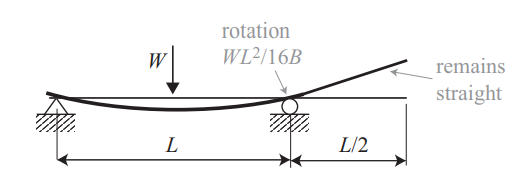
\includegraphics[width = 0.6\textwidth]{images/overhang.png}
    \caption{Overhanging beam}
    \label{fig:enter-label}
\end{figure}

Using the databook, we can observe that the rotation at the right-hand joint is equal to $\psi = \frac{WL^2}{16EI}$. Therefore, the deflection of the overhang will be:

\[ v = \frac{WL^2}{16EI} \times \frac{L}{2} = \frac{WL^3}{32EI} \]

\begin{proposition}[Non-rigid overhang]
    In the case of a beam featuring a non-rigid (loaded) piece overhanging from either support, we must superpose two separate cases:
    \begin{enumerate}
        \item Rigid beam (acting as wall support) and non-rigid overhang
        \item Non-rigid beam and rigid overhang
    \end{enumerate}
\end{proposition}

\begin{figure}[h]
    \centering
    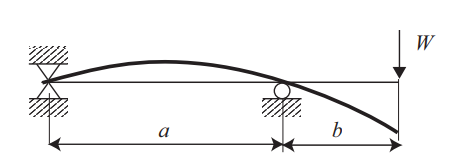
\includegraphics[width = 0.6\textwidth]{images/overhang2.png}
    \caption{Overhanging loaded non-rigid beam}
    \label{fig:enter-label}
\end{figure}

In the case where the overhang is rigid, it then means that it effectively transmits a moment $Wb$ to the beam. By the databook, the end rotation of the beam will be:

\[ \psi = \frac{Ma}{3EI} = \frac{Wba}{3EI} \]

Therefore, the deflection is:

\[ \delta_1 = \psi b = \frac{Wb^2a}{3EI} \]

Now, if the beam is rigid and acts as a support, we have the simplest case of them all, i.e. point load at the end of a cantilever, and so:

\[ \delta_2 = \frac{Wb^3}{3EI} \]

Therefore, total deflection is:

\[ \delta = \delta_1 + \delta_2 = \frac{Wb^2(a + b)}{3EI} \]

Note that this idea of linear superposition can be applied in all sorts of problems, even when we are asked to find reaction forces that are normally not indetifiable via means of equilibrium (such as a propped cantilever).

\newpage

\subsection{Stresses in elastic beams}

When analyzing stresses in elastic beams, we make two key assumptions:

\begin{enumerate}
    \item The central line (neutral axis) does not change in length
    \item All plane sections must remain plane (Euler-Bernoulli hypothesis)
\end{enumerate}

\begin{figure}[h]
    \centering
    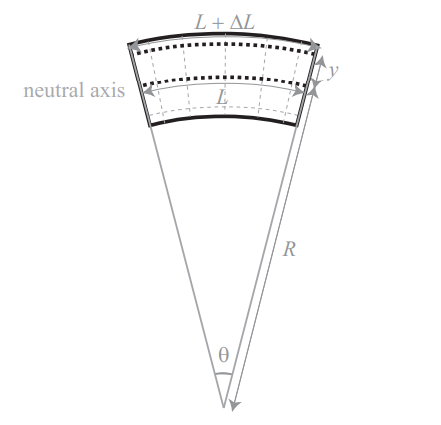
\includegraphics[width = 0.5\textwidth]{images/strains.png}
    \caption{Strain calculation}
    \label{fig:enter-label}
\end{figure}

These two assumptions allows us to consider a piece of beam of the type presented above. Therefore, by means of basic geometry:

\[ L = \theta R \]

Likewise:

\[ L \Delta L = \theta(R + y) \]

By manipulating the above, we deduce that:

\[ \frac{\Delta L}{L} = \frac{y}{R} \]

\begin{proposition}[Strain in an elastic beam]
    The strain in an elastic beam varies linearly with the curvature, i.e.:

    \[ \epsilon = \kappa y \]

    Where $y$ is the distance from the neutral axis. We will later show what the neutral axis is.
\end{proposition}

\begin{proposition}[Stress-strain equivalence]
    Due to the fact that we are assuming linear elasticity in the beams, we can determine that the stress acting at a distance $y$ from the neutral axis must be:

    \[ \sigma = E\epsilon \iff \sigma = E\kappa y \]

    Note that we can observe that for $y > 0$, $\sigma > 0$, which means that the beam is in tension. For $y < 0$, that means that $\sigma < 0$, i.e. the beam is in compression.
\end{proposition}

\begin{proposition}[Bending moment]
    The bending moment in a straight elastic beam is given by:

    \[ M = EI\Delta\kappa \]
\end{proposition}

\begin{proof}
    We are now able to finally prove this result. Consider the elemental force:

    \[ \delta T = \sigma \delta A = (E\kappa y)(\delta A) \]

    The bending moment is given by:

    \[ \delta M = y \delta A \iff \delta M = E\kappa y^2\delta A \]

    Therefore:

    \[ M = E\kappa \int_A y^2 dA \]

    We define $I := \int_A y^2dA$ as the second moment of area. Therefore:

    \[ M = EI\kappa \]
\end{proof}

Therefore, by combining the stress and moment relationship, we can now deduce that:

\[ \sigma = \frac{My}{I} \]

\begin{proposition}[Calculation of the second moment of area]
    In order to calculate the second moment of area, we must first determine where the centroid of the section is and then align our coordinate system with that axis. Then, we can simply compute the integral to find the second moment of area. The centroid is the place where:

    \[ \int_A ydA = 0 \]
\end{proposition}

\begin{proposition}[Parallel axis theorem]
    If we wish to calculate the second moment of area about a different axis, we can use the parallel axis theorem, i.e.:

    \[ I_P = I_O + Ad^2 \]

    Where $A$ is the area of the cut and $d$ is the distance between the two axes.
\end{proposition}

\subsubsection{Combined bending and axial force}

Oftentimes a beam may have to carry both a bending moment $M$ and an axial force $T$. The stress distribution can then be obtained by superposing the stresses due to both loading conditions, i.e.:

\[ \sigma = \frac{My}{I} + \frac{T}{A} \]

\begin{example}
    Compute the required axial compression $C$ in order to avoid any tensile stresses in a rectangular cross-section.

    To do this, we impose our condition:

    \[ \sigma = \frac{My}{I} - \frac{C}{A} \leq 0 \]

    The stress is greatest at $y = \frac{d}{2}$ and $I = \frac{bd^3}{12}$ for a rectangular beam. Hence:

    \[ M\frac{\frac{d}{2}}{\frac{bd^3}{12}} \leq \frac{C}{bd} \]

    Hence:

    \[ \frac{6M}{bd^2} \leq \frac{C}{bd} \iff C \geq \frac{6M}{d} \]

    If we wish to also know where this compression force needs to act, let us consider that $M = C\delta$. Hence:

    \[ C \geq \frac{6C\delta}{d} \iff 1 \geq \frac{6\delta}{d} \]

    Therefore, we can deduce that:

    \[ \delta \leq \frac{d}{6} \]

    So the force needs to act within the middle third of the section for the condition to be satisfied.
\end{example}

\subsubsection{Bending stresses in composite beams}

\begin{definition}[Composite beam]
    A composite beam is made from two or more different materials.
\end{definition}

The idea when analyzing such beams is to:

\begin{enumerate}
    \item First, convert all members into a single material, using the fact that all flexural rigidities must be the same
    \item Calculate the neutral axis position by taking moment equilibrium
    \item Calculate the second moment of area
\end{enumerate}

Now, if we wish to find the stress in one part of the beam, we simply need to use:

\[ \sigma = \frac{E_\text{current}}{E_\text{transformed}}\frac{My}{I} \]

\subsubsection{Pure bending of reinforced concrete beams}

Concrete is a material that is strong in compression, but weak in tension. Steel is equally strong in tension and compression. Therefore, the idea behind reinforced concrete is to use slender steel bars to withstand the tension due to the bending moment, and concrete to withstand compression.

\begin{figure}[h]
    \centering
    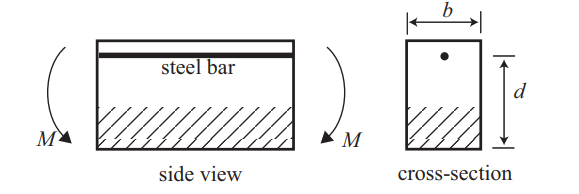
\includegraphics[width = 0.65\textwidth]{images/concrete.png}
    \caption{Reinforced concrete pure bending}
    \label{fig:enter-label}
\end{figure}

We will assume the following behaviour:

\begin{enumerate}
    \item The steel is responsible for carrying all tension
    \item The concrete is responsible for carrying all compression
    \item Any concrete in compression is equal to void/air (has no strength)
\end{enumerate}

Because anything above the neutral axis is in tension, and anything below it is in compression, we are motivated to consider the following transformation:

\begin{figure}[h]
    \centering
    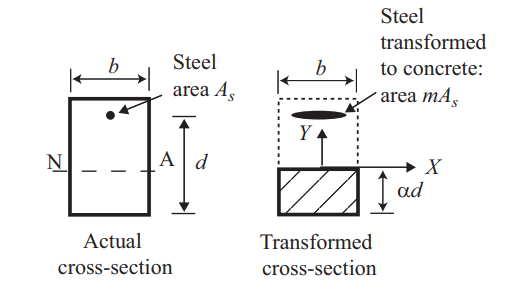
\includegraphics[width = 0.65\textwidth]{images/transform.png}
    \caption{Transformed section of reinforced concrete}
    \label{fig:enter-label}
\end{figure}

We assume that the neutral axis is at a distance $\alpha$ from the bottom of the beam. By moment equilibrium:

\[ b\alpha d \times \frac{1}{2}\alpha d = (1 - \alpha)d mA_s \]
Hence:

\[ \frac{bd^2}{2}\alpha^2 + mA_s d \alpha - mA_sd = 0 \]

Hence:

\[ \frac{bd}{2mA_s}\alpha^2 + \alpha - 1 = 0 \]

This quadratic equation can then be solved to obtain the position of the neutral axis. Furthermore, we can now use the this to compute the moment of inertia of the concrete beam, and then simply analyse it as previously.

\subsubsection{Shear stresses in beams}

Consider making a cut at a certain depth in a beam, likewise:

\begin{figure}[h]
    \centering
    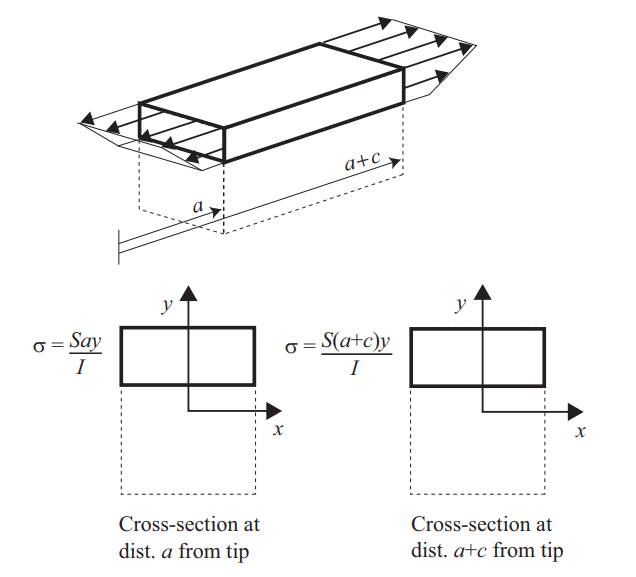
\includegraphics[width = 0.65\textwidth]{images/shear.png}
    \caption{Shear stresses}
    \label{fig:enter-label}
\end{figure}

The total longitudinal force acting at $a$ is given by:

\[ R_1 = \int_A \frac{Say}{I}dA \]

Likewise, the force acting at $a + c$ is given by:

\[ R_2 = \int_A \frac{S(a+c)y}{I}dA \]

Therefore, we must have a force balancing these two out, i.e.:

\[ Q = R_2 - R_1 = \frac{Sc}{I}\int_A ydA = \frac{ScA_c\overline{y}}{I} \]

Dividing by $c$ yields us the force per unit length:

\[ q = \frac{SA_c\overline{y}}{I} \]

Note that $A_c$ is the area of the cut surface, while $\overline{y}$ is the distance from the neutral axis of the entire beam to the centroid of the cut. If we divide by the length of the cut, we can find the shear stress:

\[ \tau = \frac{SA_c\overline{y}}{bI} \]

\newpage

\subsection{Buckling of beams}

\begin{proposition}[Hypotheses]
    To consider the buckling of a compression member, we will make a number of key assumptions:
    \begin{enumerate}
        \item The bar is pin-ended
        \item The beam is initially perfectly straight
        \item The behaviour is linear-elastic
        \item All deflections are assumed to be small
        \item Initially the beam is stress-free
    \end{enumerate}
\end{proposition}

\subsubsection{The Euler column}

Consider a simple pin-ended bar in compression. Moment equilibrium yields:

\[ M = Pv \]

Linear-elasticity yields:

\[ M = -EI\frac{d^2v}{dx^2} \]

Therefore:

\[ \frac{d^2v}{dx^2} + \frac{P}{EI}v = 0 \]

By defining $\alpha^2 = \frac{P}{EI}$, we obtain the following general solution to our differential equation:

\[ v(x) = A\sin{\alpha x} + B\cos{\alpha x} \]

The first boundary condition is $v(0) = 0$, yyielding $B = 0$. The second boundary condition is $v(L) = 0$, i.e.:

\[ A\sin{\alpha L} = 0 \]

The trivial solution is $A = 0$. However, if $A \neq 0$, then:

\[ \alpha L = n\pi \iff \frac{P}{EI} = \frac{n^2\pi^2}{L^2} \iff P = \frac{n^2\pi^2EI}{L^2}\]

The smallest value of buckling is obtained in the first mode, i.e. $n = 1$, and this is called the Euler buckling load:

\[ P_E = \frac{\pi^2 EI}{L^2} \]

\subsubsection{Fixed-end column}

Consider a column where both ends are fixed. Therefore:

\[ M = Pv - Q \]

By using linear-elasticity again, we obtain:

\[ \frac{d^2v}{dx^2} + \frac{P}{EI}v = \frac{Q}{EI} \]

By solving this equation and setting the deflection and rotation at $0$ to be $0$, and taking care to set that the deflection at $L$ must also be zero, we obtain:

\[ P = \frac{4\pi^2EI}{L^2} \]

\begin{theorem}[Effective lengths]
    If we examine carefully the mode shape for a column that is buckling, we can observe that there must always be two points of inflection. Therefore, the load at which the structure buckles will be:

    \[ P = \frac{\pi^2EI}{L_e^2} \]

    Where $L_e$ is the effective length.
\end{theorem}

Note that the above result can be obtained immediately for the fixed-end column, with $L_e = \frac{L}{2}$. 

\subsubsection{Critical stress}

Let us now examine the critical compressive stress $\sigma_{cr}$ at which a perfect strut will fail. It fails either by yielding when $\sigma_{cr} = \sigma_y$, or it will fail by buckling. The buckling stress is:

\[ \sigma_E = \frac{P_E}{A} = \frac{\pi^2E}{L^2}\left(\frac{I}{A}\right) \]

If we use the radius of gyration, we know that $I = Ar^2$. Hence:

\[ \sigma_E = \frac{\pi^2 E}{(L/r)^2} \]

Where $L/r$ is the slenderness of the column. Hence, the critical stress at failure $\sigma_{cr}$ will be the smaller of $\sigma_y$ and $\sigma_E$.

\subsubsection{Imperfections}

In practice, we are never straight, and therefore we can consider that the bar has an initial bow, defined by:

\[ v_0 = \delta_0\sin{\frac{\pi x}{L}} \]

If we consider the simple pin-ended bar, we can rewrite:

\[ Pv = M \]

The elastic law gives:

\[ M = EI\Delta\kappa \]

By accounting for the initial curvature, the governing differential equation becomes:

\[ \frac{EI}{P}\frac{d^2v}{dx^2} + v = -\left(\frac{P_E}{P}\right)\delta_0\sin{\frac{\pi x}{L}} \]

This equation can now be solved in a similar fashion as before, allowing us to deduce the critical load at which the structure will buckle.

\begin{theorem}[Perry's formula]
    The critical load at which a structure will buckle can be approximated using the formula:

    \[ (\sigma_y - \sigma_{cr})(\sigma_E - \sigma_{cr}) = \eta\sigma_{cr}\sigma_E \]
\end{theorem}

As mentioned previously, in theory the value of the critical stress is either the yield or the buckling stress. However, due to imperfections, a constant $\eta$ is introduced (experimental value). We normally use $\eta \approx 0.003 \frac{L}{r}$.

\newpage

\section{Materials}

Though they lacked the means to prove it, the ancient Greeks suspected that solids were made of discrete
atoms that packed in a regular, orderly way to give crystals. With modern techniques of X-ray and
electron diffraction and high-resolution microscopy, we know that all solids are indeed made up of
atoms or molecules, and that most (but not all) are crystalline. Most engineering metals and
ceramics are made up of many small crystals, or grains, stuck together at grain boundaries to make
polycrystalline microstructures.

\subsection{Atoms, solutions and compounds}

Atoms consist of a nucleus of protons (positive charge) and neutrons, with different elements defined by the number of protons in the nucleus. Electrons (negative charge) orbit the nucleus to balance the proton charge in discrete shells of fixed energy levels. 

\begin{definition}[The atomic number]
    For an element $X$, we define the atomic number $Z$ as the number of electrons (or protons) in the atom.
\end{definition}

\begin{definition}[The atomic weight]
    For an element $X$, we define the atomic weight $A$ to be the mass of the nucleus, which is also equal to the number of protons and neutrons.
\end{definition}

In general, we denote an element $X$ as ${}_Z X^A$. For example, for lead, we write this as ${}_{82} Pb^{207}$.

\subsubsection{Atomic size}

A surprising and important feature is that all atoms are a similar size, i.e. atomic radii are all of order
$0.1–0.2$ nm, while the atomic weight spans a factor of over $200$. In simple terms, this is because as the
number of protons and electrons increase, the electron shells are drawn in to smaller radii. Conversely, the are consequences to this:

\begin{enumerate}
    \item Mixtures of atoms of different elements (alloys) can pack efficiently into crystal lattice structures, forming solid solutions or compounds
    \item Most solid solutions will be substitutional - atoms of similar size replace one another in the lattice, e.g. $\ch{CuZn}$ in brass
    \item Only small atoms (e.g. $\ch{H}$, $\ch{C}$) form interstitial solid solutions - these atoms can fit into the gaps between metal atoms
    \item Compounds can form readily, with lattices that satisfy the required atomic fractions of the elements, or stoichiometry (e.g., $\ch{Fe3C}$, $\ch{Al2O3}$)
\end{enumerate}

\newpage

\subsection{Atomic and molecular bonding}

Atomic bonding is determined by the interaction between the outermost electrons in atoms. There are two types of bonds:

\begin{enumerate}
    \item Primary bonds: metals, ceramics, and along long-chain polymer molecules
    \item Secondary bonds: between polymer chains, and in materials such as ice
\end{enumerate}

Note that primary bonds are 100 times stronger than secondary bonds, and hence more difficult to stretch and break.

\subsubsection{Primary bonding}

\begin{definition}[Metallic bonding]
    In metallic bonding, the atoms form positively charged ions by releasing a few electrons, which then form a sea of free electrons. Bonding is done by electrostatic interaction between the ions an free electrons.

    \begin{enumerate}
        \item The bonds are equally strong in all directions - the metallic bond is non-directional
        \item Metallically bonded compounds form regular crystal lattices
        \item The free electrons are not bound to specific atoms, hence metalically bonded materials are electrical conductors
    \end{enumerate}
\end{definition}

\begin{definition}[Ionic bonding]
    In ionic bonding, electrons are transferred permanently between atoms to produce stable, oppositely charged ions, which then attract electrostatically.

    \begin{enumerate}
        \item The electrostatic forces are equal in all directions - the ionic bond is non-directional
        \item Positive and negative ions pack into regular crystal lattice structures
        \item Electrons are bound to specific ions, so ionically bounded materials are electrical insulators
    \end{enumerate}
\end{definition}

\begin{definition}[Covalent bonding]
    In covalent bonding, the electrons are shared between atoms to achieve an energetically stable number.

    \begin{enumerate}
        \item The shared electrons are associated with particular electron shells of the bonding atoms, and hence the covalent bond is directional
        \item Covalently bonded materials form regular crystal lattices (e.g. diamond), networks (e.g. glasses) or long-chain molecules (e.g. polymers)
        \item The electrons are bound to specific atoms, so covalently bounded materials are also electrical insulators
    \end{enumerate}
\end{definition}

\subsubsection{Modelling primary bonds}

Primary bonds may be modelled as stiff springs between the atoms (or ions) with a non-linear force-separation characteristic. The atoms (or ions) have an equilibrium separation $r_0$, governed by the balance between attractive and repulsive forces. At the dissociation separation, the atoms (or ions) can be separated completely. 

Atoms vibrate about the equilibrium separation with kinetic energy approximately equal to $k_BT$, where $k_B \approx 1.38 \times 10^{23}$ J/K is the Boltzmann constant, and $T$ is the absolute temperature. 

All bonds effectively break down when $k_BT$ exceeds the bond energy - at this point the material melts. Due to the strength of their primary bonds, metals and ceramics have a characteristically high melting temperature.

\begin{figure}[ht!]
    \centering
    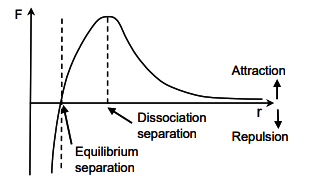
\includegraphics[width = 0.5\textwidth]{images/bond1.png}
    \caption{Force-separation characteristic}
    \label{fig:enter-label}
\end{figure}

\subsubsection{Secondary bonding}

Secondary, or Van der Waals bonds, operate at much larger atomic separation than primary bonds, and hence are much weaker. They are associated with dipoles - molecules in which the centres of positive and negative charge do not coincide.

Note that Van der Waals bonds between hydrogen atoms form the strongest dipoles and are the commonest secondary bond between polymer chains. Moreover, in secondary bonded materials (such as polymers), the bonds become ineffective at much lower thermal energies than primary bonds, giving low melting points.

\newpage

\subsection{Metal crystal structures}

Primary bonding gives a well-characterised equilibrium spacing, with stiff restoring forces. For the
purposes of packing, the atoms may be treated as hard spheres, forming a solid crystal lattice.

The great majority of the 92 stable elements are metallic, and of these, the majority (68 in all) have one of
just three simple structures: 

\begin{enumerate}
    \item Face-centred cubic (FCC)
    \item Close-packed hexagonal (CPH)
    \item Body-centred cubic (BCC)
\end{enumerate}

In total, there are 14 distinguishable three-dimensional crystal lattices, but these three structures are all that is needed for most engineering purposes.

\subsubsection{Close-packed crystal structures}

The basic building block for the first two of these structures is the
close-packed plane (i.e. the highest density of atoms arranged in a
plane is a hexagonal packing).
The close-packed directions are the straight lines through the centres
of touching atoms (there are 3 in a close-packed plane).

\begin{figure}[h]
    \centering
    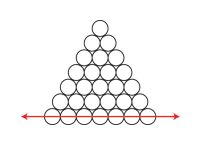
\includegraphics{images/mat1.png}
    \caption{Close-packed plane}
    \label{fig:enter-label}
\end{figure}

A 3D lattice can be built by stacking these close-packed planes – but there are 2 ways of doing it.
Around each atom there are 6 locations in which atoms can sit.
But only 3 of these can be occupied at once (“odd” or “even”).
Imagine placing a first layer above the reference layer (in either odd
or even locations). 

\begin{figure}[h]
    \centering
    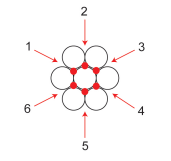
\includegraphics{images/mat2.png}
    \caption{The possible positions of atoms}
    \label{fig:enter-label}
\end{figure}

There are then two options for placing a layer
below: one using the same locations with respect to the initial layer
(giving ABA stacking), the other using the alternative locations
(giving ABC stacking), i.e. in side view:

\begin{figure}[h]
    \centering
    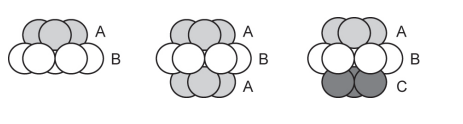
\includegraphics{images/mat3.png}
    \caption{Possible stacking for crystal lattices}
    \label{fig:enter-label}
\end{figure}

In fact, $ABC$ stacking is simply the face-centred cubic, and the $ABA$ stacking is the close-packed hexagonal. The difference is seen more clearly from their unit cells, which we will discuss just below. Both of these structures are close-packed, i.e. the spheres occupy as large a fraction of the volume as possible.

The apparently minor packing difference is of little consequence for elastic properties, but has a big influence on plastic deformation.

\subsubsection{Unit cells}

\begin{definition}[Unit cell]
    A unit cell is the smallest unit which can be replicated by translation in all directions to build up the three-dimensional crystal structure. The unit cells dimensions are called the lattice constants.
\end{definition}

Note that the unit cells are drawn with the atoms reduced in size, for clarity - remember that they touch in the close-packed directions.

\begin{definition}[The face-centred cubic (FCC) structure]
    We define the FCC structure as a cubic unit cell with one atom at each corner and one at the centre of each face. Any diagonal of any face is a close-packed direction, and the lattice constant is the length of any side of the cube.
\end{definition}

\begin{figure}[h]
    \centering
    \includegraphics[width = 0.45\textwidth]{images/mat4.png}
    \caption{Face-centred cubic structure of packed spheres showing the $ABC$ stacking}
    \label{fig:enter-label}
\end{figure}

\begin{proposition}
    For the FCC structure, the ratio of the lattice constant to the atomic radius is $2\sqrt{2}$.
\end{proposition}

\begin{proof}
    On the diagonal of any face of the FCC structure, there is one full atom and two halves. Therefore, since this is a closed-packed direction, this means that the length of the diagonal of any face of the cube is $4R$, where $R$ is the atomic radius. By Pythagoras' theorem:

    \[ a^2 + a^2 = (4R)^2 \iff 2a^2 = 16R^2 \iff \frac{a}{R} = 2\sqrt{2} \]
\end{proof}

FCC metals have the following characteristics:

\begin{enumerate}
    \item They are very ductile when pure, work hardening rapidly but softening again when annealed, allowing them to be rolled, forged, drawn or otherwise shaped by deformation processing
    \item They are generally though, i.e. resistant to crack propagation
    \item They retain their ductility and toughness t o absolute zero, something very few other materials allow for
\end{enumerate}

\begin{definition}[Close-packed hexagonal (CPH) structure]
    We define the CPH structure as a prismatic hexagonal unit cell with an atom at each corner, one at the centre of the hexagonal faces, and three in the middle. Note that this is exactly an $ABA$ type of stacking, and that the close-packed directions are the sides of the hexagonal faces.
\end{definition}

Moreover, there are two separate lattice constants in CPH - the side-length of the hexagonal base, $a$, and the height of the prism, $c$. 

\begin{figure}[h]
    \centering
    \includegraphics{images/mat6.png}
    \caption{CPH structure of packed spheres showing the $ABA$ stacking}
    \label{fig:enter-label}
\end{figure}

\begin{proposition}
    For the CPH structure, the ratio of the lattice constants $\frac{c}{a}$ is equal to $1.633$.
\end{proposition}

\begin{proof}
    Because the hexagonal sides are the close-packed directions, and because we have two halves of atoms per side, this means that $a = 2R$. Now, since two consecutive side atoms, with the middle atom and an atom at the half height form a tetrahedron, the height of this tetrahedron is just $\frac{c}{2}$. The side of the tetrahedron is then $a = 2R$, and the height of any of its faces is $h = \frac{a\sqrt{3}}{2}$. Because the height of the tetrahedron passes through the centre of mass of the opposite equilateral triangle, we can apply pythagoras do determine the height of the tetrahedron:

    \[ H^2 = h^2 - \left(\frac{a\sqrt{3}}{6}\right)^2 \iff H^2 = \frac{3a^2}{4} - \frac{3a^2}{36} = \frac{24a^2}{36} = \frac{2a^2}{3}\]

    Hence, the height of the tetrahedron is:

    \[ H = \frac{a\sqrt{2}}{\sqrt{3}} \iff c = \frac{2a\sqrt{2}}{\sqrt{3}} \]

    And then, $\frac{c}{a} \approx 1.633$, thus concluding our proof.
\end{proof}

CPH metals have the following characteristics:

\begin{enumerate}
    \item They are reasonably ductile (at least when hot), allowing them to be forged, rolled, and drawn, but in a more limited way than FCC metals
    \item Their structure makes them more anisotropic than FCC metals (i.e. crystal properties vary with direction)
\end{enumerate}

\begin{definition}[Body-centred cubic (BCC) structure]
    We define the BCC structure as a cubic unit cell with one atom at each corner and one in the middle of the cube. Note that this structure is not close-packed - it is made by stacking planes of atoms in a square array (not hexagonal). Also, the close-packed directions are the cube diagonals, and the lattice constant is the cube's side.
\end{definition}
    
\begin{proposition}
    For the BCC structure, the ratio of the lattice constant to the atomic radius is $\frac{4R}{\sqrt{3}}$. 
\end{proposition}

\begin{proof}
    Since the cube diagonal is the close-packed direction and because its length is $4R$, we can apply Pythagoras' theorem:

    \[ (4R)^2 = a^2 + (a\sqrt{2})^2 = 3a^2 \iff 16R^2 = 3a^2 \]

    Therefore:

    \[ \frac{a}{R} = \frac{4R}{\sqrt{3}} \]
\end{proof}

BCC metals have the following characteristics:

\begin{enumerate}
    \item They are ductile, particularly when hot, allowing them to be rolled, forged, drawn or otherwise shaped by deformation processing
    \item They are generally tough, and resistant to crack propagation
    \item They become brittle at low temperatures. The change happens at the “ductile-brittle transition temperature”, limiting their use below this
\end{enumerate}

\subsubsection{Grain structure}

Metal components are commonly manufactured by casting – solidification of a liquid poured into a shaped mould. The solidification mechanism involves the formation of many solid crystalline nuclei, which grow by attachment of atoms to the crystal at the interface between liquid and solid. This is explored further in the IB Materials course. For now, we note that solidification is completed when adjacent crystals impinge on one another. But because the orientation of the packing in each crystal is random, there is a misfit in the atomic packing at the interface between two crystals. The individual crystals are called grains, and the region of imperfect packing is called a grain boundary – see the figure below.

\begin{figure}[h]
    \centering
    \includegraphics[width = 0.35\textwidth]{images/mat7.png}
    \caption{Grain boundary illustration}
    \label{fig:enter-label}
\end{figure}

\newpage

\subsection{Theoretical density of metals}

We will now introduce a way of calculating the theoretical density of any metal.

\subsubsection{Atomic packing fraction}

\begin{definition}[Atomic packing fraction]
    We define the atomic packing fraction as the fraction of space occupied by the atoms in an unit cell.
\end{definition}

\begin{example}
    Let us determine the atomic packing fraction of the FCC structure. We know that $a = 2\sqrt{2}R$, and therefore the total volume of the unit cell is:

    \[ V = a^3 = 16\sqrt{2}R^3 \]

    In total, we have $8 \times \frac{1}{8} + 6 \times \frac{1}{2} = 4$ atoms per unit cell. Therefore, the volume occupied by the atoms is:

    \[ V_0 = 4 \times \frac{4\pi R^3}{3} \]

    Hence, the atomic packing fraction is then:

    \[ f = \frac{V_0}{V} \approx 0.74 \]
\end{example}

Note that for the CPH, the atomic packing fraction is the same as for the FCC, however for the BCC it is lower, proving that the BCC is not a close-packed structure.

\subsubsection{Evaluation of theoretical density}

The density of crystalline materials depends directly on the number of atoms per unit volume, and the atomic mass of the atoms.

\begin{proposition}[Theoretical density]
    For a unit cell with $i$ types of different atoms with $n_i$ atoms of each type and with atomic mass $A_i$, the theoretical density is:

    \[ \rho = \frac{\sum_i n_iA_i}{V_cN_A} \]

    Where $V_c$ is the volume of the cell and $N_A$ is Avogadro's number, i.e. $N_A \approx 6.02 \times 10^{23}$ mol$^{-1}$.
\end{proposition}

\newpage

\subsection{Interstitial space}

\begin{definition}[Interstitial space]
    An interstitial space (or hole) is the space between the atoms or molecules. The FCC, CPH and BCC structures contain interstitial space of two sorts: tetrahedral and octahedral. These are defined by the arrangement of the surrounding atoms, as shown in the figures below.
\end{definition}

\begin{figure}[h]
    \centering
    \includegraphics[width = \textwidth]{images/mat8.png}
    \caption{Interstitial holes in various unit cell structures}
    \label{fig:enter-label}
\end{figure}

Interstitial holes are important because small foreign atoms can fit into them. For FCC and CPH structures, the tetrahedral hole can accommodate, without strain, a sphere with a radius of 0.22 of that of the host. The octahedral holes are almost twice as large. Atoms are in reality somewhat elastic, so that foreign atoms that are larger than the holes can be squeezed into the interstitial space. Note that to find the diameter of the sphere, we simply calculate the distance between two base atoms and subtract the length they occupy (i.e. $2R$).

Interstitial solute atoms are particularly important for carbon steel, which is iron with carbon in some of the interstitial holes. Iron is BCC (at room temperature), and only contains tetrahedral holes (shown in Figure (c) above). These can hold a sphere with a radius 0.29 times that of the host, without strain. Carbon will go into these holes, but because it is a bit too big, it distorts the crystal structure. It is this distortion that gives carbon steels much of their strength. 

Another significant factor in carbon steels is the difference in maximum hole size between FCC and BCC. Iron transforms to FCC (at temperatures around $800^\circ$C, depending on the C content). This means that much more carbon will “dissolve” in FCC (at high temperature) than in BCC (at room temperature) – this is central to the heat treatment and strengthening of carbon steel (covered in Part IB). Interstitial holes appear in another context below: they give a way of understanding the structures of many ceramic compounds: oxides, carbides and nitrides.

\begin{example}
    Compute the diameter of the largest sphere that will fit in the octahedral hole in the FCC structure.

    To do so, we first recall that the close-packed direction is the cube face diagonal. Therefore, the diagonal is $4R$, and hence the side of the FCC is just $a = 2\sqrt{2}R$. This is also the base length in the octahedral hole. Therefore, the diameter is just:

    \[ d = 2\sqrt{2}R - 2R = 2(\sqrt{2} - 1) \]
\end{example}

\newpage

\subsection{Ceramic crystals}

Technical ceramics are the hardest, most refractory structural materials. The ceramic family also includes many functional materials (semiconductors, piezoelectrics, ferromagnetic etc.). Their structures often look complicated, but can mostly be interpreted as atoms of one type, arranged on a simple FCC, CPH or BCC lattice, with the atoms of the second type (and sometimes a third) inserted into the interstitial holes of the first lattice. There are four main crystal structures for engineering ceramics: diamond cubic, halite, corundum and fluorite. Two of these are illustrated here, to demonstrate the underlying principles.

\subsubsection{The diamond-cubic (DC) structure}

The hardest ceramic of all is diamond, of major importance for cutting tools, polishes and scratch-resistant coatings. Silicon and germanium, the foundation of semiconductor technology, have the same structure. Carbon, silicon and germanium atoms have a 4-valent nature – each atom prefers to have 4 nearest neighbours, symmetrically placed around them. The DC structure achieves this. 

The figure below shows the DC unit cell. If you first ignore the numbered atoms, the remainder form an FCC lattice; the atoms numbered 1-4 are then additional atoms located in half of the tetrahedral interstitial spaces. As the tetrahedral hole is far too small to accommodate a full-sized atom, the others are pushed further apart, lowering the density.

\begin{figure}[h]
    \centering
    \includegraphics[width = 0.25\textwidth]{images/mat9.png}
    \caption{The diamond-cubic structure}
    \label{fig:enter-label}
\end{figure}

Silicon carbide (like diamond) is very hard, and its structure is closely related. Carbon lies directly above silicon in the periodic table, it has the same crystal structure and is chemically similar. So it is no surprise that silicon carbide, with the formula \ch{SiC}, has the diamond structure with half the carbon atoms replaced by silicon. 

\begin{figure}[h]
    \centering
    \includegraphics[width = 0.25\textwidth]{images/mat10.png}
    \caption{The structure of silicon carbide}
    \label{fig:enter-label}
\end{figure}

\subsubsection{Oxides with the Corundum structure}

A number of oxides have the chemical formula $\ch{M2O3}$, among them alumina, $\ch{Al2O3}$. The oxygen, the larger of the two ions, is close-packed in a CPH stacking, and the M atoms occupy two thirds of the octahedral holes in the lattice.

\begin{figure}[h]
    \centering
    \includegraphics{images/mat11.png}
    \caption{The M atoms of the corundum structure}
    \label{fig:enter-label}
\end{figure}

\subsubsection{Glasses}

When crystalline materials melt, the atoms lose their regular packing but are still loosely held together; on solidification, crystals usually form readily. Glasses are all based on silica, SiO2, for which crystallisation is difficult. In the solid state silica usually has an amorphous (or glassy) structure, and only crystallises if cooled very slowly. The difference is shown schematically in two dimensions below.

\begin{figure}[h]
    \centering
    \includegraphics{images/mat12.png}
    \caption{Glass structures}
    \label{fig:enter-label}
\end{figure}

Amorphous structures give transparency, with the colour and refractive index of the glass readily
being customised by alloying.

\newpage

\subsection{Polymer microstructure}

Polymers are long-chain molecules of carbon (typically $10^4$ – $10^6$ atoms). Along the chains are side bonds to atoms of H, Cl, F, or groups of atoms such as a methyl group, $\ch{CH3}$. The simplest polymer (polyethylene) is formed by polymerisation of a basic $\ch{CH2}$ monomer into a chain molecule.

Primary bonding between the C atoms is by strong covalent bonds – both along the chains, and at cross-links (where two chains are bonded together). Secondary bonding acts between the chains (via the side-groups) by weak Van der Waals bonds.

\begin{figure}[h]
    \centering
    \includegraphics[width = 1\textwidth]{images/mat13.png}
    \caption{Polymer bonds}
    \label{fig:enter-label}
\end{figure}

Polymers are inherently low in density (similar to that of water): they are made of light elements (carbon, hydrogen), and the low packing density of the molecules leaves more “free space” in the structure

\subsubsection{Microstructure in polymers}

There are three main classes of polymer: thermoplastics, thermosets and elastomers. In all cases the long-chain molecules pack together randomly, giving an amorphous “spaghetti-like” microstructure. The classes are then distinguished by the detail in the molecular architecture, in particular, whether the extent of covalent cross-linking between chains.

\begin{definition}[Thermoplastics]
    Thermoplastics contain no cross-links (covalent bonds between the chain molecules), but are divided into two sub-groups: amorphous and semi-crystalline.
\end{definition}

\begin{figure}[h]
    \centering
    \includegraphics{images/mat14.png}
    \caption{Thermoplastics}
    \label{fig:enter-label}
\end{figure}

In amorphous thermoplastics, the long-chain molecules are arranged entirely at random, with occasional entanglement points between chains. At these points there is no additional bonding, but they do restrain the deformation and sliding of the molecules. Semi-crystalline thermoplastics are partly amorphous, and partly ordered in crystalline regions (known as “spherulites”).

\begin{definition}[Elastomers and thermosets]
    Elastomers contain a small number of cross-links, between simple chain molecules. Natural rubber is an example, in which the cross-links are provided by sulphur. Further cross-linking can be triggered in service (e.g. by UV light or ozone), leading to polymer degradation. Thermosets, in contrast, have extensive cross-links between chains.
\end{definition}

\begin{figure}[h]
    \centering
    \includegraphics{images/mat15.png}
    \caption{Elastomers and thermosets}
    \label{fig:enter-label}
\end{figure}

\newpage

\section{Introductory solid mechanics}

\subsection{Constitutive response. Elastic deformation}

We are now going to move our attention towards the elastic deformation of solids.

\begin{definition}[Poisson's ratio]
    Recall that in uniaxial tension, the material gets longer and thinner, and the lateral contraction and the tensile extension are proportional. For this reason, we define Poisson's ratio as:

    \[ \nu = -\frac{\text{Lateral strain}}{\text{Tensile strain}} \]
\end{definition}

Note that lateral strain is not due to volume conservation, but it actually reflects the way atomic bonds deform under a certain load. For crystalline materials, Poisson's ratio is within the range of $0.2 - 0.33$, for porous solids it is null, and for elastomers it is approximately $0.5$, which is the highest theoretical value it can have.

\begin{proposition}[Hooke's law in 3D]
    Consider a unit cube of material (representing any volume element in a uniformly loaded body), under a general set of stresses $(\sigma_1, \sigma_2, \sigma_3)$ on its three axes. Therefore, the strains for each axis are:

    \[ \epsilon_1 = \frac{1}{E}(\sigma_1 - \nu\sigma_2 - \nu\sigma_3) \]
    \[ \epsilon_2 = \frac{1}{E}(-\nu\sigma_1 + \sigma_2 -\nu\sigma_3) \]
    \[ \epsilon_3 = \frac{1}{E}(-\nu\sigma_1 -\nu\sigma_2 + \sigma_3) \]
\end{proposition}

\begin{proof}
    To prove Hooke's law in 3D, we first realize that the state of stress forms a linear system, and hence superposition is applicable. Consider the first axis (labeled 1), and consider the sole effect of $\sigma_1$ on it. The strain in the $1$ direction is:

    \[ \epsilon_1 = \frac{\sigma_1}{E} \]

    This is the tensile strain, as the stress is applied in the same direction. By the definition of Poisson's ratio, the lateral strain is given by:

    \[ \epsilon_{2,3} = -\nu\epsilon_1 = -\frac{\nu\sigma_1}{E} \]

    These are the strains imposed on each axis by the stress $\sigma_1$. By repeating the same procedure for each individual stress, and then by using linear superposition, Hooke's law in 3D is proved.
\end{proof}

\begin{proposition}[Dilatation]
    When materials strain elastically, their volume changes. We define the dilatation as the volumetric strain, i.e.:

    \[ \Delta = \frac{\Delta V}{V_0} = \epsilon_1 + \epsilon_2 + \epsilon_3 \]
\end{proposition}

\begin{proof}
    Consider a unit cube, and a general strain state $(\epsilon_1, \epsilon_2, \epsilon_3)$, where the strains are much smaller than 1. Initial cube dimensions are $(1, 1, 1)$, and final dimensions are $(1 + \epsilon_1, 1 + \epsilon_2, 1 + \epsilon_3)$. Therefore, the final volume is:

    \[ V = (1 + \epsilon_1)(1 + \epsilon_2)(1 + \epsilon_3) = 1 + \epsilon_1 + \epsilon_2 + \epsilon_3 + \mathcal{O}(\epsilon^2) \]

    Since the initial volume is $V_0 = 1$, by applying the definition of the dilatation, the proof is complete.
\end{proof}

\begin{definition}[Hydrostatic stress]
    A state of hydrostatic stress is when all three normal stresses are equal, i.e.:

    \[ \sigma_1 = \sigma_2 = \sigma_3 \]

    An example of this is under an external pressure $p$:

    \[ \sigma_1 = \sigma_2 = \sigma_3 = -p \]
\end{definition}

\begin{proposition}[Bulk modulus]
    The bulk modulus $K$ is defined as:

    \[ K = \frac{\text{Hydrostatic stress}}{\text{Volumetric strain}} = \frac{E}{3(1 - 2\nu)} \]
\end{proposition}

\begin{proof}
    Since the state of stress is hydrostatic, we may assume that:

    \[ \sigma_1 = \sigma_2 = \sigma_3 = \sigma \]

    By Hooke's law in 3D, we deduce that the strain in any of the axes' directions is:

    \[ \epsilon = \frac{1}{E}(\sigma - \nu\sigma - \nu\sigma) = \frac{\sigma}{E}(1 - 2\nu) \]

    Since the volumetric strain is $\Delta = \epsilon_1 + \epsilon_2 + \epsilon_3 = 3\epsilon$, because we are under hydrostatic loading, we deduce that the dilatation is:

    \[ \Delta = 3\epsilon = \frac{3\sigma}{E}(1 - 2\nu) \]

    By applying the definition:

    \[ K = \frac{\sigma}{\Delta} = \frac{E}{3(1 - 2\nu)} \]
\end{proof}

Previously, we have defined normal stress as the force per unit area carried perpendicular to a plane within the material. However, it is useful to define the shear stress.

\begin{definition}[Shear stress]
    The shear stress $\tau$ is defined as the force per unit area carried parallel to a plane within the material.
\end{definition}

This type of stress distorts the shape of a volume element, rather than changing its axial dimensions - for this reason it is useful to define the shear strain. Because the changes are small, we can define it as the approximate angle (in radians) made with that specific plane.

\begin{definition}[Shear strain]
    The shear strain is defined as $\gamma = \frac{w}{l_0}$. Note that since we postulate that the modifications are small, we can approximate $\gamma \approx \tan{\gamma}$.
\end{definition}

\begin{definition}[Shear modulus]
    The shear modulus $G$ characterizes the elastic stiffness in shear:

    \[ G = \frac{\text{Shear stress}}{\text{Shear strain}} = \frac{\tau}{\gamma} \]

    By means of elastic analysis, we can further deduce that:

    \[ G = \frac{E}{2(1 + \nu)} \]

    This result is, however, non-trivial, and is beyond the scope of this course.
\end{definition}

\subsection{Plastic properties}

The typical response for a ductile metal is, as previously shown: (1) linear elastic behavior, (2) elastic limit - material reaches the yielding limit $\sigma_y$, (3) permanent plastic strain, (4) tensile strength and (5) necking - deformation localizes, and specimen fails.

Previously we have defined the elastic stored energy as the area of the stress-strain curve until $\sigma_y$. This is equal to:

\[ V = \frac{1}{2}\sigma_y\epsilon_y = \frac{\sigma_y^2}{2E} \]

Likewise, the plastic work per unit volume is the area under the stress-strain curve, excluding the final elastic contribution, i.e.:

\[ W = \int \sigma_n d\epsilon_n \]

Although in elastic deformation, the volume is not conserved, it is, however, conserved in plastic deformation (until the point of necking). Therefore:

\[ Al = A_0l_0 \]

\begin{definition}[Hardness]
    In compression testing, the hardness of a material is defined as:

    \[ H = \frac{\text{Load}}{\text{Projected area of indent}} \approx 3\sigma_y \]

    Note that this result is purely empirical.
\end{definition}

\begin{proposition}[True stress]
    The true stress for an uniaxial load is:

    \[ \sigma_t = \sigma_n(1 + \epsilon_n) \]

    Where $\sigma_n$ and $\epsilon_n$ are the nominal stress and strain, respectively.
\end{proposition}

\begin{proof}
    Because volume is conserved during plastic deformation, $A_0l_0 = Al \iff \frac{A_0}{A} = \frac{l}{l_0}$.
    By definition, $\sigma_t = \frac{F}{A}$ and $\sigma_n = \frac{F}{A_0}$. Hence:

    \[ \sigma_t = \frac{A_0}{A}\sigma_n = \frac{l}{l_0}\sigma_n \]

    Because $\epsilon_n = \frac{l - l_0}{l_0} \iff \frac{l}{l_0} = 1 + \epsilon_n$. Therefore:

    \[ \sigma_t = \sigma_n(1 + \epsilon_n) \]

    Therefore, true stress is higher than nominal stress for positive stress values.
\end{proof}

\begin{proposition}[True strain]
    The true strain of a material can be obtained by summing together all the individual contributions of strain, i.e. each $\frac{dl}{l}$. Therefore:

    \[ \epsilon_t = \int_{l_0}^l \frac{1}{l}dl = \ln{\frac{l}{l_0}} \]

    However, since $\frac{l}{l_0} = 1 + \epsilon_n$, we deduce that:

    \[ \epsilon_t = \ln{\left(1 + \epsilon_n\right)} \]

    Therefore, true strain is smaller than nominal strain for positive strain values.
\end{proposition}

\subsection{Stress analysis}

Under uniaxial tension (or compression), all elastic materials strain laterally (due to Poisson's ratio). Let us now consider different cases when analyzing stresses is important.

\subsubsection{Constrained deformation}

\begin{proposition}[Constrained deformation]
    Consider a cube of material fitted into a square-section slot in a rigid plate, and loaded with a compressive stress $\sigma_1$. We impose a constraint in the third direction, namely $\epsilon_3 = 0$ Because the material is only loaded in the first direction, $\sigma_2 = 0$. Note that the same cannot be said about $\sigma_3$, since the wall induces a compressive stress in the material. By Hooke's law in 3D:

    \[ \epsilon_3 = 0 = \frac{1}{E}(-\nu\sigma_1 + \sigma_3) \]

    This means that:

    \[ \sigma_3 = \nu\sigma_1 \]

    In the first direction:

    \[ \epsilon_1 = \frac{1}{E}(\sigma_1 - \nu\sigma_3) \]

    By combining both equations, we obtain:

    \[ \epsilon_1 = \frac{\sigma_1(1 - \nu^2)}{E} \]

    Therefore, we observe that:

    \[ E' = \frac{\sigma_1}{\epsilon_1} = \frac{E}{1 - \nu^2} \]

    The material effectively changes Young's modulus (it becomes stiffer) as to adjust for the constraint we imposed.
\end{proposition}

\subsubsection{Thermal deformation}

\begin{proposition}[Thermal strain]
    We define the thermal stress for a material in terms of the thermal expansion coefficient $\alpha$ and the absolute change in temperature $\Delta T$ as:

    \[ \epsilon = \alpha\Delta T \]

    The thermal stress can then be deduced by $\sigma = E\epsilon = E\alpha\Delta T$.
\end{proposition}

We must also note that in problems where measuring the thermal stress is key, it must be important to note the following relationship:

\[ \epsilon_t + \epsilon_e + \epsilon_p = 0 \]

Meaning that the thermal, elastic and plastic strains all cancel each other out.

\begin{proposition}[Constrained surface layers]
    Consider two different interfaces (surfaces) with thermal expansion coefficient $\alpha_1$ and $\alpha_2$. Then, the induced total strain will be:

    \[ \epsilon_t = (\alpha_1 - \alpha_2)\Delta T \]

    If $\alpha_1 > \alpha_2$, the top layer goes into tension. Otherwise, it goes into compression.
\end{proposition}

\newpage

\section{Microstructure and properties}

In this section of the course, we will discuss the microstructural properties of materials, and analyze these in terms of elasticity and plasticity.

\subsection{Manipulation of elastic properties}

As previously shown, in crystalline materials, atoms pack in a regularly repeating lattice structure. Most metals are commonly used as alloys, although some can also be used in pure form.

\begin{definition}[Ceramic]
    A ceramic material is a compound of a metal with silicon (Si) or other non-metals (such as $O_2$, $C$ or $N_2$).
\end{definition}

\begin{proposition}[Elastic response of metals and ceramics]
    Primary bonds can be thought of as stiff springs. The gradient of the $F = F(r)$ response is called the bond stiffness $S$. For a small displacement from equilibrium:

    \[ F = Su \]

    The strain will also be equal to $\epsilon = \frac{u}{r_0}$, where $r_0$ is the equilibrium spacing of atoms. We can also obtain the stress:

    \[ \sigma = \frac{Su}{r_0^2} \]

    And hence, the Young's modulus is:

    \[ E = \frac{\sigma}{\epsilon} = \frac{S}{r_0} \]

    Therefore, the Young's modulus of a component directly reflects the bond stiffness and is a material property. The atomic response $F - u$ is linear, giving what we call as linear elasticity at a macro scale.
\end{proposition}

\begin{definition}[Alloys]
    Alloys are mixtures of elements (typically metals), forming solid solutions and compounds.
\end{definition}

From the hard sphere model, solid solutions and compounds will form densities between those of the pure elements. Solid solutions contain a mixture of different bond stiffnesses  ($A-A, A-B, B-B$), and hence the Young's modulus of $A-B$ solutions will lie somewhere between pure $A$ and pure $B$. Note that compounds have stiffer bonds, and therefore a higher modulus - the stronger chemical bond is a major reason as to why the compound forms.

\subsubsection{Polymer elasticity}

We first note that we distinguish between three classes of polymers:

\begin{enumerate}
    \item Thermoplastics: polyethylene, polyvinylchloride, polypropylene, polystyrene
    \item Thermosets: epoxies, phenolics, polyurethane
    \item Elastomers: rubbers, neoprene
\end{enumerate}

Note that of the three classes of polymers mentioned above, only thermoplastics can be recycled. We will understand why this is the case in the following sections.

\begin{definition}[Glass transition temperature]
    In crystalline materials and glasses, the breaking of primary bonds by thermal energy gives a well-defined property, also known as the melting temperature $T_m$. In polymers, the weaker secondary (Van der Waals) bonds are overcome by thermal energy at a lower temperature. This is known as the glass transition temperature $T_g$. This is the temperature at which the polymer becomes rigid and glassy.
\end{definition}

\begin{definition}[Amorphous polymers]
    We say that a polymer is amorphous if its molecular structure is entangled, i.e. it is formed by randomly distributed atoms.
\end{definition}

Above the glass transition temperature, the behaviour of polymers differs:

\begin{enumerate}
    \item Amorphous thermoplastics melt to a viscous liquid (the entangled molecules slide over one another)
    \item In semi-crystalline thermoplastics, the amorphous regions melt, but the crystalline regions survive up until a higher melting point $T_m$, above which a viscous liquid forms
    \item In elastomers and thermosets, the secondary bonds melt at $T_g$, but the cross-links do not - on heating, the polymer does not melt, but decomposes or burns
\end{enumerate}

\subsubsection{Manipulating elastic properties}

\begin{definition}[Foam]
    A foam is a porous solids. Note that porous, cellular solids are found extensively in nature (e.g. wood).
\end{definition}

\begin{proposition}[Young's modulus for a foam]
    Consider an idealised unit of material where the elastic response is dominated by the bending of the solid ligaments. Then:

    \[ \frac{E_f}{E_s} = \left(\frac{\rho_f}{\rho_s}\right)^2 \]

    Where $(E_f, \rho_f)$ are the foam's properties, and $(E_s, \rho_s)$ are the properties of the solid material used.
\end{proposition}

\begin{definition}[Composite]
    Composite materials combine two different materials to produce new property profiles, exploiting separate qualities of the individual components.
\end{definition}

Composites are defined by the volume fraction $V_f$ of one of the components, which represents the volume of that component relative to the total volume. The density of the composite can be approximated by:

\[ \rho_c = \rho_f V_f + \rho_m (1 - V_f) \]

\begin{proposition}[The Voigt-Reuss equations]
    Consider a composite made of a particulate fiber and a matrix. Then, we can deduce the upper and lower bounds for the predicted Young's Modulus. The upper bound is given by the longitudinal modulus (parallel to layers):

    \[ E_c = V_fE_f + (1 - V_f)E_m \]

    The lower bound is given by the transverse modulus (perpendicular to layers);

    \[ E_c = \left(\frac{V_f}{E_f} + \frac{1 - V_f}{E_m}\right)^{-1} \]

    Note that this is true for isotropic materials (equivalent response in all directions).
\end{proposition}

\subsection{Manipulation of plastic properties}

\begin{definition}[Strength]
    We define the strength of a material as the nominal stress at the elastic limit.
\end{definition}

There are different ways in which materials respond to tensile tests:

\begin{enumerate}
    \item Brittle materials (in tension): fracture occurs at the elastic limit due to cracks, giving a tensile strength
    \item Brittle materials (in compression): crushing occurs, giving a compressive stress - this is due to the fact that cracks form, and by compressing the material, the gaps are closed
    \item Ductile materials (e.g. metals), in either tension and compression, have their strength defined as the yield stress $\sigma_y$
\end{enumerate}

\subsubsection{Atomic basis of plasticity in crystalline materials}

The atomic bonding in crystalline materials is strong and primary: metallic, ionic or covalent. Elastic deformation displaces atoms by a fraction of their equilibrium spacing, whereas plastic deformation involves relative movement of material over very large multiples of the atomic spacing.

\begin{proposition}[Ideal strength of crystalline materials]
    The ideal strength is the notional tensile stress which would cause simultaneous rupture of the inter-atomic bonds across the whole sample.  This occurs when the load on the atoms reaches the maximum in the atomic force-separation curve. As the material deforms, atoms must overcome a periodic energy potential:

    \[ U(x) = U_0\cos{\frac{2\pi x}{b}} \]

    Where $b$ is called the Burgers vector. We know that in a force field, $\mathbf{F} = -\nabla\mathbf{V}$. Therefore:

    \[ F(x) = \frac{2\pi U_0}{b}\sin{\frac{2\pi x}{b}} \]

    If we label $N_x$ as the number of atoms per unit area, then the maximum shear stress required to overcome the energy barrier is:

    \[ \tau_0 = \frac{2\pi U_0N_x}{b} \]

    The magnitude of this shear force must depend on the material itself. At small strains, the force required to displace atoms follows linear elasticity, and the shear strain is:

    \[ \gamma = \frac{x}{b} \]

    Since the shear modulus $G$ is defined as $G = \lim_{\gamma \to 0} \frac{\partial\tau}{\partial\gamma}$, we conclude that:

    \[ \tau_0 = \frac{G}{2\pi} = \frac{E}{4\pi(1 + \nu)} \]

    The maximum shear stress occurs when $\sigma = 2\tau$ (proved in an earlier section). Therefore, the ideal stress is:

    \[ \sigma_y = \frac{E}{2\pi(1 + \nu)} \]
\end{proposition}

Note that this is only an estimate of the ideal strength of a material. However, in reality, the strength of a material is orders of magnitude lower than this estimate - our goal is to now investigate why this occurs.

\begin{definition}[Dislocations]
    A dislocation is a line defect in a crystal which can move over a slip-plane in the lattice under an applied shear stress.  Dislocations concentrate the applied stress on a small proportion of the bonds, so plastic deformation takes place one row of atoms at a time at a stress which is much lower than the ideal strength. Yielding therefore occurs by very many tiny increments of shear between the blocks of crystal on either side of the slip planes.  The magnitude of the incremental displacement is called the Burgers vector $b$. 
\end{definition}

To accommodate  for this atomic displacement, part of the interface between the top and bottom half of the crystal slipped, and part has not. The top half contains an extra half-plane of atoms. 

Consider a dislocation moving right through a block of material. This gives a net displacement between the material above and below the slip plane. The slip step produced by the passage of one single dislocation is the Burgers vector, and dislocations enable incremental slip by extending a few  bonds at a time. This is specifically why the stress required is much less than the ideal strength.

There are different types of dislocations:

\begin{enumerate}
    \item Edge dislocations - the shear stress and Burgers vector are both at right angles to the dislocation line, but they all move in the same direction
    \item Screw dislocations - the shear stress and Burgers vector are  both parallel to the dislocation line, but they move perpendicular to one another
    \item Mixed dislocations - these are curved dislocations, varying between pure edge and pure screw
\end{enumerate}

Note that the same slip step is produced for both edge and screw dislocations. For mixed dislocations, the net effect remains a slip step in the direction of the shear stress.

\begin{proposition}[Dislocation resistance per unit length]
    The dislocation resistance per unit length (force per unit length) is given by:

    \[ f = \tau b \]

    Where $\tau$ is the shear stress and $b$ is the Burgers vector.
\end{proposition}

\begin{proposition}[Line tension]
    Atoms around a dislocation are displaced from their equilibrium spacing, and thus have a higher energy. The energy (per unit length, actually a force) $T$ is given by the elastic stress-strain field around the dislocation core:

    \[ T = \frac{1}{2}Gb^2 \]

    Where $G$ is the shear modulus and $b$ is the Burgers vector.
\end{proposition}

\begin{proposition}[Dislocation pinning]
    When a gliding dislocation meets obstacles in its slip plane, it is pinned by the obstacles and is forced to bow out between them, increasing the resistance per unit length, and an additional shear stress $\Delta\tau$ is required to overcome this resistance.

    The total force on an obstacle is given by:

    \[ F = 2T\cos{\theta} \]

    We say that an obstacle is weak if $\theta > 0$. Otherwise, we say that the obstacle is strong.

    We know that the resistance is $f = \tau b$. Therefore, the additional resistance encountered is:

    \[ \Delta f = \Delta \tau b \]

    For a projected length $L$ of dislocation between obstacles, the force is:

    \[ F = \Delta\tau bL \]

    However, the force is $F = 2T\cos{\theta}$. Therefore:

    \[ 2T\cos{\theta} = \Delta\tau bL \iff Gb^2\cos{\theta} = \Delta\tau bL \]

    Therefore, the additional shear stress required to surpass an obstacle is:

    \[ \Delta\tau = \frac{Gb}{L}\cos{\theta} \]

    Where $G$ is the shear modulus, $b$ is the Burgers vector, $L$ is the obstacle spacing, and $\cos{\theta}$ is the obstacle strength.
 \end{proposition}

\begin{definition}[Casting]
    Casting is a process by which solidification occurs by nucleation and growth of tiny solid crystals. These will randomly grow until they impinge, forming grains.
\end{definition}

\begin{definition}[Re-crystallisation]
    Grains reform in the solid state by heat treatment following the previous deformation.
\end{definition}

Between the remote shear stress $\tau$ and the shear stress needed to move dislocations $\tau_y$, the following relationship holds: $\tau = \frac{3}{2}\tau_y$. By taking note that $\sigma_y = \frac{\tau}{2}$ at $\frac{\pi}{4}$ inclination, then:

\[ \sigma_y = 3\tau_y \]

\begin{definition}[Dislocation length per unit volume]
    We define the dislocation length per unit volume as:

    \[ \rho_d = \frac{L}{V} \]

    Where $L$ is the length of dislocations and $V$ is the volume of the sample. Note that dislocation density rises with strain, reducing the spacing and increasing the resistance.
\end{definition}

\begin{definition}[Work hardening]
    Work hardening is a process by which materials are deformed (e.g. rolling, wire drawing, cold rolling) to increase the dislocation density while shaping the product. This increases the strength of the material.
\end{definition}

In work hardening, the spacing between dislocations is given by:

\[ L = \frac{1}{\sqrt{\rho_d}} \]

Because of this, the increase in yield stress is proportional to $Gb\sqrt{\rho_d}$.

\begin{definition}[Solid solution hardening]
    Solid solution hardening is a process by which solute atoms are added into the material (interstitial solid solutions) to provide a weak obstacle to dislocations, which bow out until the line tension pulls the dislocation past the solute atom. This is generally done through casting.

    Note that the increase in yield stress is proportional to $\sqrt{C}$, so the spacing between dislocations is proportional to $\frac{1}{\sqrt{C}}$.
\end{definition}

\begin{definition}[Precipitation hardening]
    When compounds are distributed as small particles within a lattice, they provide pinning points for dislocations. Particles can be introduced in different ways, but the hardening is referred to generally as precipitation hardening. The increase in yield stress is on the order of $10 \times$, and these particles act as strong obstacles for dislocations ($\theta = 0$).

    The increase in yield stress is:

    \[ \Delta\sigma_y = \frac{3Gb}{L} \]
\end{definition}

\subsubsection{Failure of polymers}

Polymer strength is determined by the ability of the chain molecules to unravel and slide, temperature, strain-rate, crystallinity (in thermoplastics) and cross-links (in thermosets and elastomers). The potential barrier approximation we have done above works well for polymers, however note that it is not a fair approximation due to the fact that we have assumed primary bonding - polymers have secondary bonds.

\begin{proposition}[Behaviour of thermoplastics]
    Below $T_g$, thermoplastics are elastic-brittle, and above $T_g$, they are elastic-plastic.

    \begin{enumerate}
        \item If $T < T_g$, we have an elastic-brittle response - chain sliding is limited, and brittle fracture occurs from inherent flaws in the material. There is little to no ductility
        \item If $T > T_g$, chain mobility increases around $T_g$ as secondary bonds melt, and yielding takes place by crazing, shear yielding or cold drawing
    \end{enumerate}

    In crazing, microcracks open in tension, bridged by stiff fibres of material with aligned molecules, preventing immediate fracture. In shear yielding, shear bands form and are stabilised by the alignment of molecules, giving greater ductility. In cold drawing, necking occurs - but the neck is stable: the molecules align in the neck and strengthen it, so the neck spreads along the specimen - there is perfect plastic deformation until the point of fracture.
\end{proposition}

\begin{proposition}[Behaviour of thermosets and elastomers]
    Below $T_g$, both thermosets and elastomers are elastic-brittle. However, above $T_g$, for thermosets there is limited shear yielding (deforms slightly plastically, then fractures). Elastomers are non-linear elastic - they feature very high elastic strains until failure, and have little or no ductility - past the elastic limit, they fail by brittle fracture.
\end{proposition}

\newpage

\section{Fracture mechanics}

In this section of the course, we will now cover fracture mechanics, and later on - Weibull statistics.

\subsection{Brittle fracture}

\begin{proposition}[Stress concentration factor]
    Consider an elliptical crack in the middle of a rectangular region, of major axis $a$. Then, if we apply a remote stress $\sigma_0$, the maximum stress is concentrated at the edge (tip) of the flaw and is given by:

    \[ \frac{\sigma_{\text{max}}}{\sigma_0} = 1 + 2\sqrt{\frac{a}{r}} > 1 \]

    Where $2a$ is the crack length and $r$ is the radius of curvature of the tip. This equation is only valid for blunt features (circular/elliptical holes). Note that if we are dealing with a circle, $a = r$ and this implies that the maximum stress is $3\sigma_0$.

    Note that this gives an approximation of the maximum stress at the edge of a crack - this shows us that the crack suffers from much larger stresses than the remote applied stress to the sample.
\end{proposition}

\begin{proposition}[Strain energy release rate]
    The strain energy release rate is the rate at which the stored elastic energy is released with respect to the creation of new crack area. It is given by:

    \[ G = \frac{\pi\sigma_0^2a}{E} \]

    Where $2a$ is the crack length  and $\sigma_0$ is the remote stress.
\end{proposition}

\begin{proof}
    As previously shown, the stored elastic energy per unit volume is:

    \[ U = \frac{\sigma_0^2}{2E} \]

    Therefore, the energy released when the crack extends by $da$ must be given by $dW = UdV$. Hence:

    \[ dW = \frac{\sigma_0^2}{2E} 4\pi a t da = \frac{2\sigma_0^2 \pi a t da}{E} \]

    Since the crack area is $dA = 2t da$, by equating $G = \frac{dW}{dA}$, we obtain the required formula.
\end{proof}

\begin{definition}[Stress intensity factor]
    By the analisys of the stress field around a crack, we can deduce that:

    \[ \sigma_{yy} = \frac{K}{\sqrt{2\pi x}} \]

    Where $K$ is the stress intensity factor and $x$ is the distance from the $Y-Y$ axis. It is a measure of the crack tip loading. This dependence is often put in the form:

    \[ K = Y\sigma\sqrt{\pi a} \]

    Where $Y$ is a dimensionless constant and $a$ is a unit of length.
\end{definition}

\begin{example}
    The Materials databook gives values of $Y$ for many different geometries. For instance, for a centre crack of length $2a$, we can define $K$ as:

    \[ K = \sigma\sqrt{\pi a} \]

    Where we use $a$ as the radius (semi-length) of the feature. Note, again, that $K$ is only defined for sharp features.

    For an edge crack, we use the total length of it (in a semi-infinite plane):

    \[ K = 1.12\sigma\sqrt{\pi a} \]

    Note that here we use the full length of the feature.
\end{example}

\begin{proposition}[Uniting the stress and energy approaches]
    Fracture is expected when $K$ and $G$ reach a critical value, the critical stress intensity factor $K_{IC}$ and the critical strain energy release rate $G_{IC}$. Note that $K_{IC}$ is often named the fracture toughness, whereas $G_{IC}$ is the fracture energy. Therefore, for fracture:

    \[ K \geq K_{IC}    \text{    and    }    G \geq G_{IC} \]

    Moreover, the following relationship holds:

    \[ K = \sqrt{EG} \]

    This is also true for $K_{IC}$ and $G_{IC}$.
\end{proposition}

Note that the subscript $I$ denotes that these critical values are for the mode I of crack loading. Note that Mode I is the opening mode, where the crack surface is displaced normal to the surface. Mode II is the sliding or in-plane shear mode, where the two surface slide over each other. Mode III is the tearing mode, where shearing is done in another plane rather than the tangent one.

\subsection{Ductile fracture}

A central issue in fracture of ductile materials concerns the plastic flow at the crack tip. Plasticity raises the radius of curvature at the crack tip and reduces the stress concentration effect.

The stress concentration at the crack tip:

\begin{enumerate}
    \item Stimulates plasticity
    \item Blunts the crack tip
    \item Reduces the stress (usually to $\approx \sigma_y$)
    \item Has extensive energy absorption
\end{enumerate}

\begin{proposition}[Crack tip process zone]
    The size of the process zone is given by:

    \[ r_P = \frac{K_{IC}^2}{\pi\sigma_y^2} \]

    Note that the stress intensity factor $K$ can be used to predict fracture if the process zone size $r_P$ is small compared with the specimen and crack dimensions. Otherwise, when $r_P$ is on the order of the crack length, the stresses in the process zone are no longer characterized only by $K$.
\end{proposition}

In general, as $\sigma_y$ increases, $K_{IC}$ goes down. At lower temperatures, dislocations are less mobile, and the fracture toughness falls. Note that the fracture toughness $K_{IC}$ is the resistance to crack propagation, which is also equal to the loss in potential energy.

\subsection{Micro-mechanisms of fracture}

\begin{proposition}[Fracture in metals]
    Plasticity concentrates stress on inclusions, nucleating voids that grow and coalesce, ultimately causing ductile fracture.
    In brittle fracture, the energy absorbed is likely to be relatively low, and the fracture surface shows little evidence of extensive plastic flow.
\end{proposition}

\begin{proposition}[Fracture in ceramics]
    Fracture in ceramics is dominated by their brittle nature. Failure starts from flaws or pores which are introduced during processing. Fracture may occur either through grains (transgranular) or along the grain boundaries (intergranular).

    Tensile failure occurs from the "worst flaw". We can, therefore, deduce that:

    \[ \sigma_t = \frac{K_{IC}}{Y\sqrt{\pi a_{\text{max}}}} \]

    Note that, as before, we use the full length of an edge crack or the semi-length of a centre crack.

    Compressive failure is initiated in Mode II (in-plane shear) - this will occur on the planes of maximum shear stress, which are those at $\frac{\pi}{4}$ to the loading axis. Failure under compression requires a much higher driving force than in tension - mainly due to frictional work being done behind the crack tip as asperities on the crack flanks slide over each other. This is also why the compressive strength of brittle materials is usually much greater than the tensile strength. Therefore, ceramics are weak in tension, and strong in compression.
\end{proposition}

\end{document}
